%!TEX TS-program = xelatex
%!TEX encoding = UTF-8 Unicode
%!BIB program = bibtex

\documentclass[oneside, 11pt, letterpaper]{marl}

\proposaltitle{\doublespacing 
	Modern Generative Methods for Music Transcription \\
	{\textcolor{red}{[A draft compiled at \currenttime, \today]}}
}

\threecommittee
{Professor Juan Pablo Bello, Chairperson}
{Professor Robert Rowe}
{Doctor Eric J. Humphrey}

\degree{Doctor of Philosophy}
\degreedate{\the\year}

\author{\href{mailto:jongwook@nyu.edu}{Jong Wook Kim}}
\program{Program in \href{http://steinhardt.nyu.edu/music/technology/}{Music Technology}}
\department{Department of \href{http://steinhardt.nyu.edu/music/}{Music and Performing Arts Professions}}
\university{\href{http://www.nyu.edu/}{New York University}}
\crest{}%\includegraphics[width=3in]{NYUlogoLarge2597}}
\submittedtext{Submitted in partial fulfillment\\
  of the requirements for the degree of\\
  Doctor of Philosophy in the\\
  \href{http://steinhardt.nyu.edu/}{Steinhardt School of Culture, Education, and Human Development}}

% turn of those nasty overfull and underfull hboxes
\hbadness=10000
\hfuzz=50pt
\makeindex

%\addbibresource{library/library.bib}
\renewcommand{\doublespacing}{\setstretch{1.5}}

\begin{document}

\sloppy
\widowpenalty=10000
\clubpenalty=10000

%: ----------------------- generate cover page ------------------------
%\setstretch{1.2}
\maketitle  % command to print the title page with above variables
% \makecopyright
% 
% Thesis Abstract -----------------------------------------------------


%\begin{abstractslong}    %uncommenting this line, gives a different abstract heading
\begin{abstracts}        %this creates the heading for the abstract page

Put your abstract or summary here, if your university requires it.

\end{abstracts}
%\end{abstractlongs}


% ---------------------------------------------------------------------- 


\doublespacing
% % Thesis Dedictation ---------------------------------------------------

\begin{dedication} %this creates the heading for the dedication page

To the Flying Spaghetti Monster.

\end{dedication}

% ----------------------------------------------------------------------

% 
% this file is called up by thesis.tex
% content in this file will be fed into the main document

\chapter*{Acknowledgements}

Sweet sweet sweet roll croissant candy souffle pie chocolate bar.
Pudding candy carrot cake sweet halvah. 
Ice cream ice cream tiramisu jelly-o chupa chups chupa chups carrot cake. 
Donut tootsie roll pie pudding icing muffin candy canes. 
Cupcake tootsie roll croissant chocolate applicake croissant macaroon gummi bears. 
Muffin icing icing toffee jelly beans toffee lemon drops. 
Cookie chocolate cake topping carrot cake chocolate bar jujubes sweet roll.

\singlespacing

%: ----------------------- contents ------------------------
% levels are: 0 - chapter, 1 - section, 2 - subsection, 3 - subsubsection
\setcounter{secnumdepth}{3} % organisational level that receives a numbers (NYU Steinhardt recommends level 0, which is pretty hideous)
\setcounter{tocdepth}{1}    % print table of contents for level 2

{
	\small 
	\tableofcontents            % print the table of contents
	%\addcontentsline{toc}{section}{continued}
	%: ----------------------- list of figures/tables ------------------------
	
	%\clearpage
	%\listoftables                   % print list of tables
	\clearpage
	\listoffigures                  % print list of figures
}

\chapterbegin

% % this file is called up by thesis.tex
% content in this file will be fed into the main document

\newacronym{tcap}{TCAP}{Toffee chocolate apple pie}


\newglossaryentry{Chupa chups}
{
  name={chupa chups},
  description= {Powder fruitcake ice cream ice cream brownie biscuit ice cream ice cream}
}

% 
\chapter*{}

\begin{quote}
``Marshmallow wafer oat cake carrot cake sugar plum gummi bears jujubes marzipan.''

\end{quote}

\vspace{1in}
\hspace{2in}
-Willy Wonka, {\it Midnight in the Garden of Good and Evil.}

\chapterbegin
\mainmatter
\doublespacing

%: ----------------------- subdocuments ------------------------

%!TEX root = ../dissertation.tex
% this file is called up by thesis.tex
% content in this file will be fed into the main document

%: ----------------------- introduction file header -----------------------
% the code below specifies where the figures are stored
\graphicspath{{1-introduction/figures/}}

\chapter{Introduction}
\label{ch:introduction}

As listening is a core constituent of human perception, an essential component of artificial intelligence is \emph{machine listening}.
The purpose of machine listening research is to enable computers to process and understand sounds as humans do.
In recent years, there have been an unprecedented amount of successes in the field of \emph{machine learning}, a near-synonym to artificial intelligence with a connotation of statistical and/or probabilistic methodologies, which redefined what a computer vision or natural language processing systems can do and made previously unimaginable applications such as autonomous driving and a superhuman StarCraft-playing AI into reality.

In this context, this thesis focuses on improving the machine understanding of music in order to automatically transcribe music, which largely remains an unsolved problem despite decades of research.
The recent rapid development in \emph{deep learning} research, however, hints at many new possibilities for improving the performance or even achieving human-level accuracy in music transcription.

\section{Statement of Problem}\label{sec:statement}

\begin{figure}
	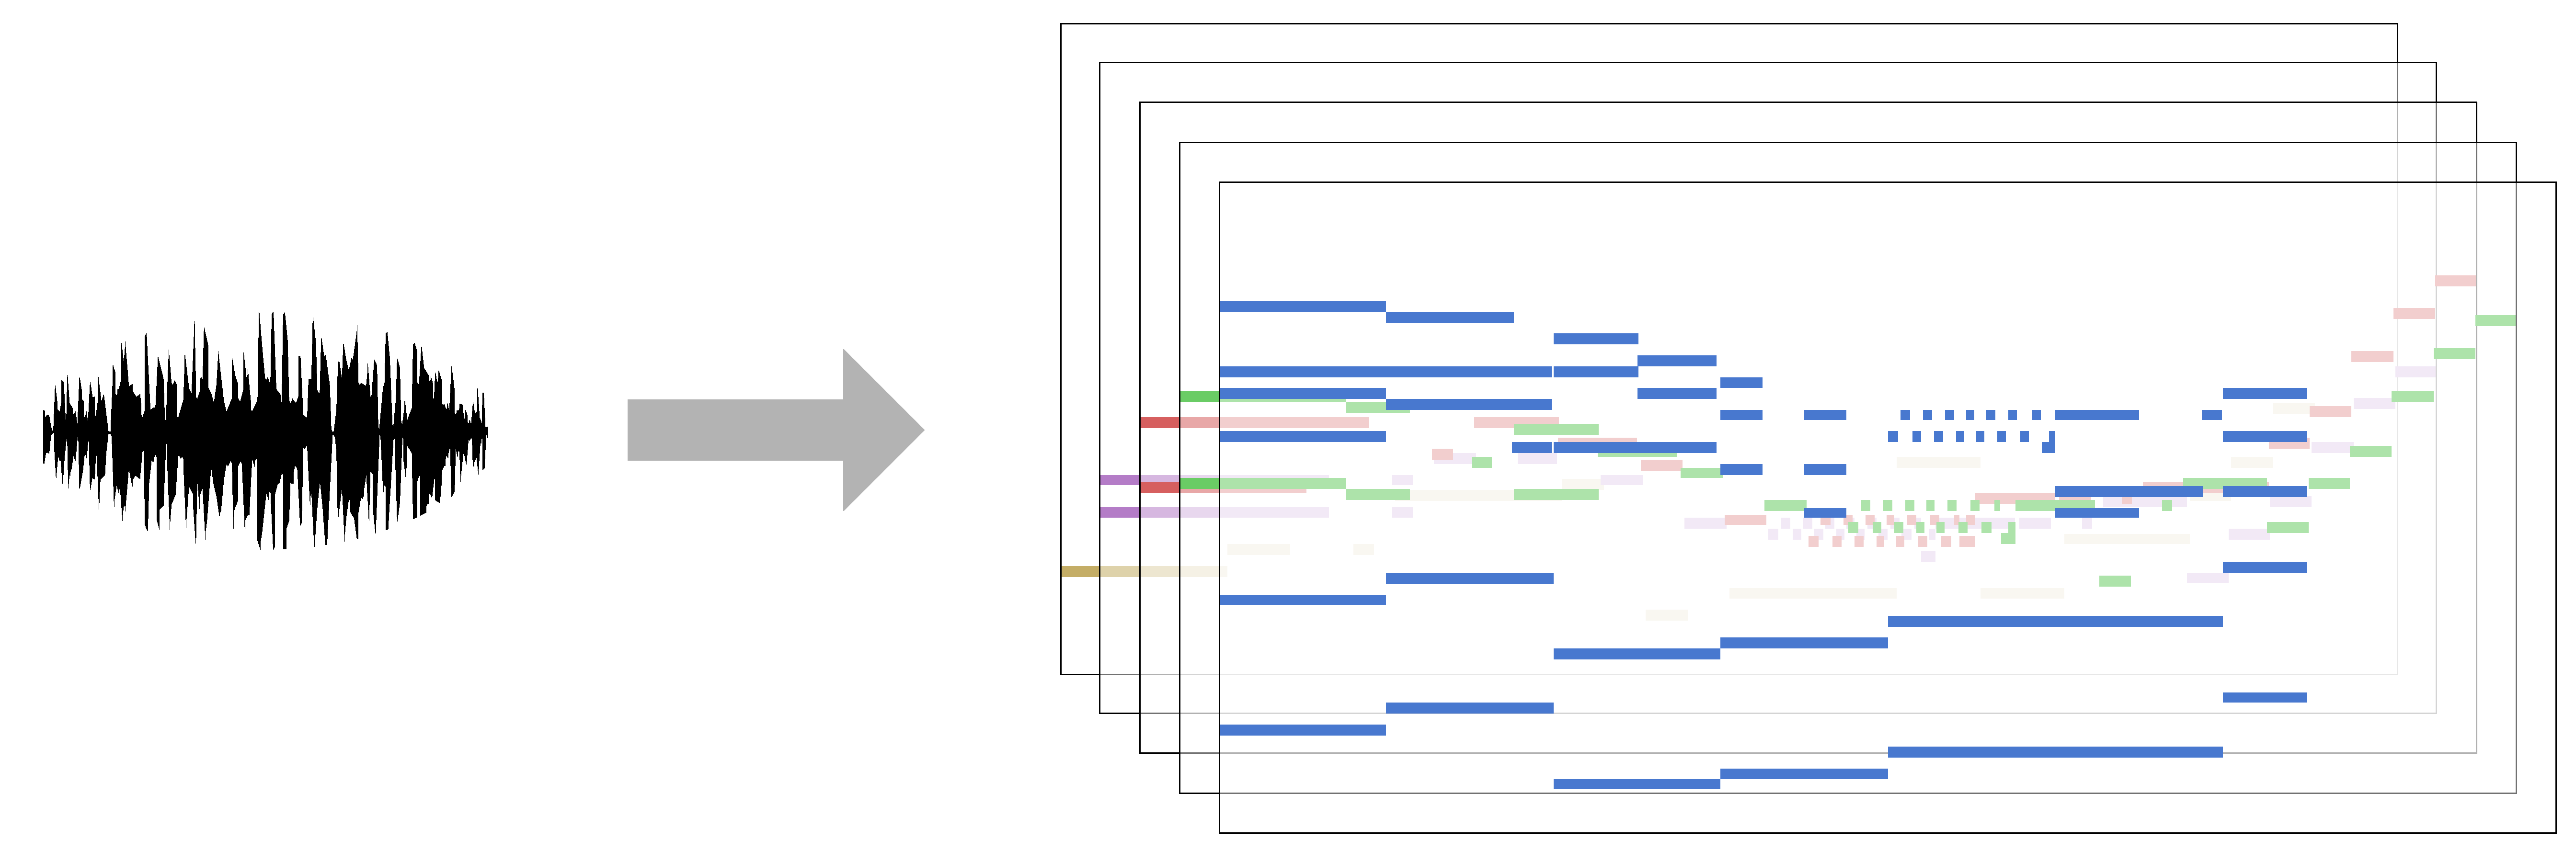
\includegraphics[width=\textwidth]{march-transcription.pdf}
	\caption{The automatic music transcription setup to be used in this thesis. Using per-instrument piano-roll representations is easier for machines to process, and avoids variability and subjectivity that may arise from symbolic and textual notations.} 
	\label{fig:transcription-to-piano-rolls}
\end{figure}

\emph{Automatic music transcription} (AMT) refers to an automated process that can identify musical events in the input audio and convert them into musical notations.
Historically, the definition of automatic music transcription varied by author, usually in terms of the form of the output representation.
In earlier works \cite{moorer1977transcription,piszczalski1977transcription}, the final output of the transcription system was to be the common music notation, i.e. a score, while later literature generalizes the problem by defining it as ``the analysis of an acoustic musical signal so as to write down the pitch, onset time, duration, and source of each sound that occurs in it" \cite{klapuri2006transcription} or ``the process of converting an acoustic musical signal into some form of musical notation" \cite{benetos2013amt}.
This thesis adopts per-instrument piano-rolls as the resulting representation of automatic music transcription, as shown in Figure \ref{fig:transcription-to-piano-rolls}, and defers the ``piano-roll to score" conversion as an out-of-scope task, which involves higher-level nontrivial tasks such as tempo and meter tracking, key signature detection, and music structure identification.
This can be justified since it allows the transcription model to focus on source separation and multi-pitch tracking, which are already highly challenging problems \cite{cemgil2006generative}.


To perform automatic music transcription, various properties of musical events, such as pitch, timbre, harmony, beats, etc., need to be defined and extracted from the audio.
In this sense, the setup of AMT is \emph{discriminative} in nature, meaning that it aims to identify different attributes from given audio, as opposed to \emph{generative} models concerning how to construct audio signals according to given conditions about those attributes.
Meanwhile, when a generative model is jointly trained with an encoder, it can learn to generate data samples from a small number of latent factors, while the encoder learns to extract those factors from the audio in a compact representation, as depicted in Figure \ref{fig:autoencoder}.
Recently, with the increased capacity of machine learning models and hardware, many \emph{deep generative models} have been proposed and shown to be capable of processing high-dimensional multimedia data.
Furthermore, significant research efforts have been made towards learning disentangled representation of data, meaning that the latent factors contain meaningful information that can be easily separated and isolated.
To this end, the goal of this thesis is to study representation learning methods powered by deep generative models, to obtain disentangled information from audio signals that can achieve better performance in music transcription.

\begin{figure}[t]
	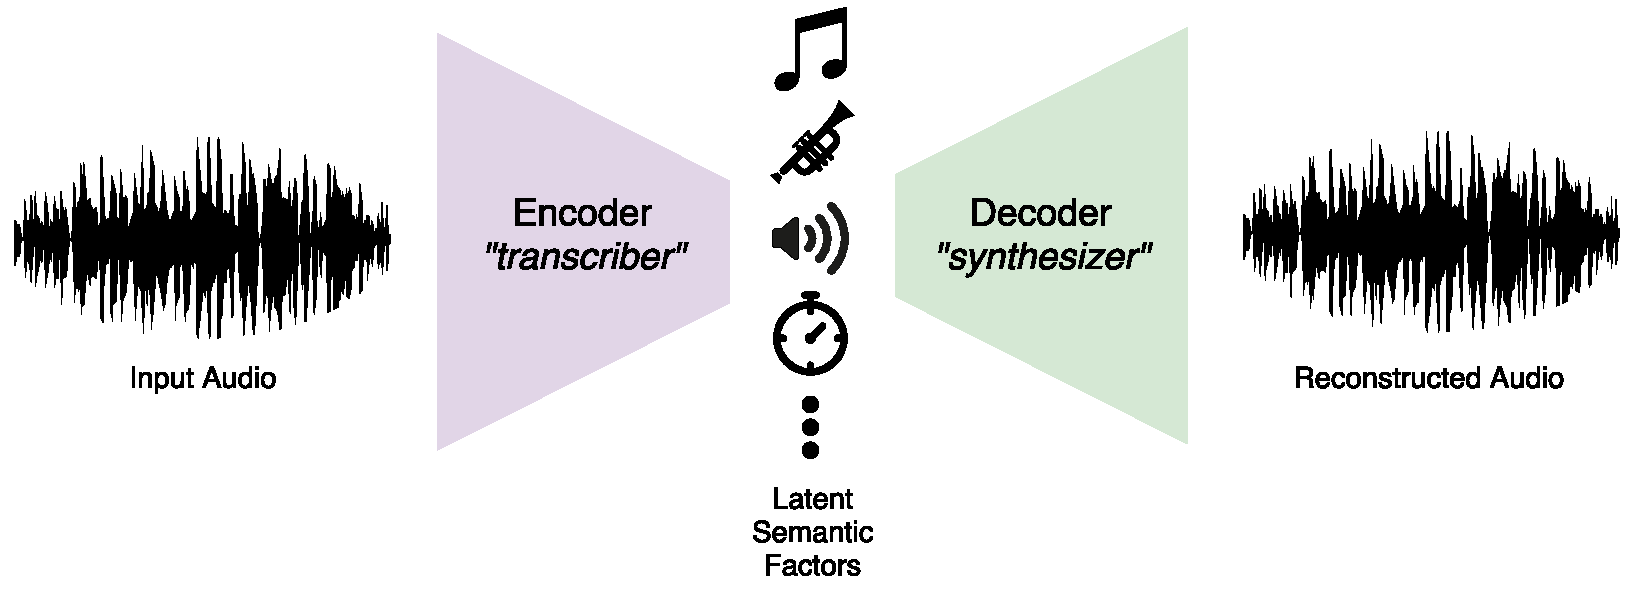
\includegraphics[width=\textwidth]{autoencoder.pdf}
	\caption{A generative model has to know all of necessary information required to reconstruct the audio data, including pitch, timbre, loudness, and duration. Generative models can be jointly trained with an encoder that finds those semantic information, giving a transcriber-synthesizer pair.}
	\label{fig:autoencoder}
\end{figure}

\section{Research Questions}\label{sec:subproblems}

To achieve the goal of improving music transcription with generative models, several research questions needs to be addressed. This thesis considers the following questions regarding the proposed approach towards automatic music transcription.

\vspace{1em}

\begin{enumerate}
\item What kinds of deep models and representations can be used for effectively extracting pitch from audio?
\item How does the choice of datasets affect the accuracy and the generalizability of a trained model?
\item How can we encode the concept of timbre in a way that is useful for music synthesis and transcription?
\item How can a transcription model make informed predictions incorporating the knowledge of music theory?
\item Can a music synthesizer component based on a deep generative model be used to improve music transcription?
\end{enumerate}

\vspace{1em}

We aim to address each of these questions in the technical chapters of the thesis.
Through extensive experimental analysis in each chapter, we draw the conclusion on the effectiveness of deep generative models in the context of automatic music transcription.


\section{Limitations}\label{sec:limitations}

Because of the sophisticated and open-ended nature of automatic music transcription, it is necessary to define the scope of the tasks and data that this thesis will be concerned with.
The purpose of this section is to define those limitations in terms of the scope of music that the proposed AMT system can process, the required capability of symbolic music processing, and the need for perceptual studies regarding the validity of AMT systems.


\subsection{Scope of Music}

Music signals typically contain both harmonic and percussive sources. 
From a signal processing point of view, harmonic sounds are quasi-periodic and contain energy only at certain frequencies, roughly at the multiples of the fundamental frequency, whereas percussive or highly inharmonic sounds have aperiodic frequency spectra in which it is not possible to define a fundamental frequency.
Consequently, transcription models for harmonic sounds and percussive sounds require different techniques according to their nature.


This thesis will limit the focus on the transcription of harmonic sounds and therefore use the per-instrument piano roll notation (Figure \ref{fig:transcription-to-piano-rolls}) as the output representation.
This is a realistic trade-off to make, because of a number of reasons.
First, learning to simultaneously model harmonic and percussive sounds is a harder problem both conceptually and computationally.
Secondly, it is possible to plug a harmonic-only model into a pipeline consisting of HPSS (harmonic-percussive source separation) and a percussion transcription model as an alternative to a comprehensive approach.
Lastly, polyphonic transcription is considered to be the most difficult problem in the domain of automatic transcription, and it is sensible to tackle this as a standalone problem in the simplest possible setup.
Excluding percussive sounds will disallow using most of pop music tracks as-is, but multi-track datasets can still be utilized since they contain each track separately.


Additional limitations should be considered on the types of the instruments and their sound variations.
Depending on the instrument, the same score could be performed using a variety of expressive techniques, such as vibrato, tremolo, pizzicato, and the usage of mutes or harmonics, among others.
In order to accurately produce a piano roll transcription that is invariant to such techniques, the model has to be trained to classify them as nonessential information, requiring the availability of datasets with the annotations for those techniques.
While an ideal model should learn those concepts as humans do, too much timbral or temporal variation for an instrument will prevent the model from learning a consistent representation corresponding to the instrument.
Therefore, for the immediate purpose of this thesis, distributions of music signals that do not contain too much of said variations will be employed.


\subsection{Symbolic Processing of Notes}

As mentioned and justified in the problem statement (Section \ref{sec:statement}), by choosing per-instrument piano rolls as the output of transcription, concerns of symbolic music processing such as beat quantization and score typesetting are excluded from the scope of this study.
The difference between a piano roll output and a full human-readable score output becomes apparent when we compare the piano rolls in Figure \ref{fig:transcription-to-piano-rolls} with Figure \ref{fig:wedding-march-score}, which is the original score from which the piano rolls are plotted.
There are many aspects in producing the score output that are highly subjective and difficult to derive a consistent evaluation metric from, such as the interpretation of legatos or staccatos and the aesthetic choices for typesetting, providing an additional justification for using the piano roll notation.


\begin{figure}
	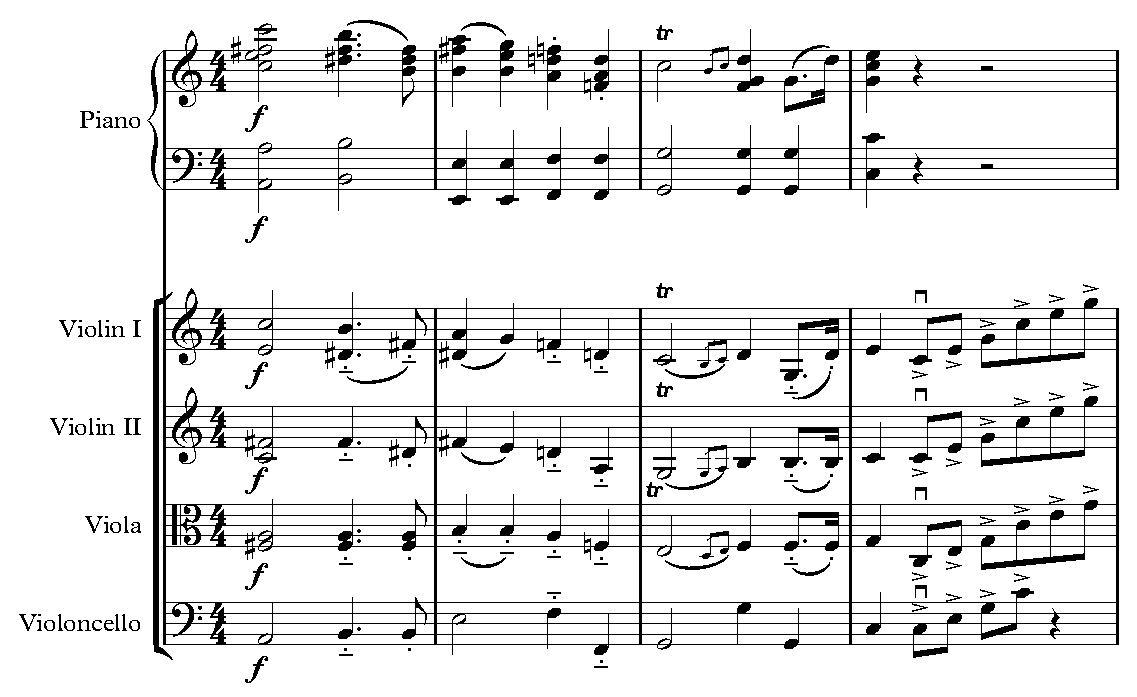
\includegraphics[width=\textwidth]{march-score.pdf}
	\caption{The full score notation of the music used to build the piano rolls in Figure \ref{fig:transcription-to-piano-rolls}. To fully recover this level of notations from the audio, the transcriber has to make many additional decisions than for the piano rolls, such as determining the key signature, time signature, clefs, dynamics, trills, bowing instructions, etc.}\label{fig:wedding-march-score}
\end{figure}


The MIDI file format is suitable for encoding data equivalent to per-instrument piano rolls, consisting of multiple tracks of \texttt{note\_on} and \texttt{note\_off} events with the corresponding timestamps.
MIDI will therefore be a supported output format of the proposed AMT system in addition to the piano roll representations, which can also be conveniently played back by media player software.
Music typesetting software such as Sibelius or Finale can render a MIDI file into score notation using the metadata in the file as well as some heuristics for beat quantization.
However, the readability of the score rendered from a transcribed MIDI file is limited, due to imperfect transcription and the absence of metadata such as the time and key signature.



\subsection{On the Need for Perceptual Studies}

This study of automatic music transcription is entirely quantitative and does not involve subjective tests on human participants.
We only aim to discover the systematic relations between audio signals and corresponding note sequences present in the datasets we use for training.
However, music is essentially a perceived notion, and thus are the core qualities of sound --- pitch, timbre, and loudness --- which are the output of automatic transcription.
For this reason, manually annotating polyphonic music is an error-prone process, where any two annotators may produce drastically different annotations.
Although this problem of inaccuracy and subjective difference is often overcome by using a ground-truth dataset synthesized from known frequency information, the gap still persists between what a model can learn from synthesized audio and how it will respond to real-world sounds.
This thesis uses both kinds of datasets, from synthesized and recorded audio signals, and thus the real-world applicability of each of the proposed models should be carefully examined.

The goal of automatic transcription is at a lower level than for tasks such as  chord recognition and melody tracking, which may incur even more subjective disagreements caused by the imprecise definitions of chords and melodies.
Being directly related to the physical concept of fundamental frequency, pitch is relatively precisely defined in this sense, and formulating automatic music transcription as an audio-to-piano-roll conversion mostly eliminates the ambiguity that exists in chord recognition and melody tracking.
There exist some cases where the mathematical definition of fundamental frequency still cannot be applied for all pitched sounds, such as the Shepard tone \cite{shepard1964circularity} where the pitch of a harmonic sound fails to be consistently mapped to a fundamental frequency.
However, disregarding these few edge cases, this study assumes that the piano roll notation can convey an objective transcription for many practical purposes, allowing us to postulate AMT as a mathematical problem which does not require experiments on human subjects.

\section{Need for Study}

The nature of music transcription is multifold; to create a complete transcription, one has to identify all instruments, onsets, dynamics, and the pitch traces for every instrument present in the music, and it would still be far from achieving the human-level accuracy.
The need for this study arises naturally, not only because this is an intriguing problem in the intersection of music and technology that has remained unsolved for decades, but also because the solution to this problem can provide practical benefits to many applications.

In order to bolster the need for this study, a few of such applications are introduced in this section, followed by discussions on the advantages of employing generative models as a means of better capturing musical semantics.
A brief perspective on AMT is presented in the context of wider AI research, followed by the organization of the chapters.


\subsection{Applications of Automatic Music Transcription}\label{sec:applications}

Many applications of the techniques in the realm of automatic music transcription is on interactive music systems.
\citeA{vercoe1984performer} proposed a quest for a \emph{synthetic performer}, which can listen, perform, and learn in the context of live performance.
Relevant sub-fields include automatic \emph{real-time accompaniment} \cite{dannenberg1985accompaniment} based on dynamic programming was one of the first successful demonstrations of AMT techniques, and \emph{Score following}, a general term referring to the synchronization of a computer with a performer playing a known score \cite{orio2003following}.
An offline music-to-score matching algorithm can also be applied to intelligent audio editors \cite{dannenberg2003following}.

\emph{Music recommender systems} can combine many kinds of information for improved music retrieval and personalization \cite{celma2010music}.
Content-based music recommender systems can utilize not only the metadata but also the audio content, and methods using timbral \cite{magno2008recommendation}, temporal \cite{li2007recommender}, and tonal features \cite{lu2009recommendation} have been introduced.
These music recommender systems can be further improved when the complete information on each domain is made available through AMT.

AMT system can help create databases for query-by-humming \cite{ghias1995humming} by automatically estimating melody annotations, where users can retrieve music by humming an excerpt of the song.
Such databases can also facilitate large-scale musicological analyses \cite{abdallah2015british}, as well as the development of computer-aided music composition \cite{agostini2013aid} that incorporates musicological knowledge.


\subsection{Generative Modeling for Fully Capturing Semantics}

Being ``generative'' means that a model is capable of generating new samples in the domain of the original data.
Generation in the symbolic domain creates new musical scores, and a generative model in the audio domain creates audio waveforms.
These two kinds of generative systems are familiar to computer music artists and are referred to as algorithmic composition \cite{fernandez2013ai} and sound synthesis \cite{cook2002synthesis} models.
This thesis defines the term ``generative model'' more specifically, as a model that can learn the distribution of provided data and can sample new samples in the original distribution.
This differs from the term ``generative'' used in computer music in a sense that it aims to accurately model the probability distribution and learn to regenerate the real-world audio to be used in music transcription, rather than focusing on the artistic aspects of generating new kinds of sounds and music.

By learning to generate data using fewer parameters than the scale of the dataset, a model has to discover the underlying natural features from the distribution of data.
In music transcription, these features correspond to the musical concepts such as pitch, timbre, and rhythm.
Philosophically, this idea follows what Richard Feynman once wrote on his blackboard, \emph{``What I cannot create, I do not understand''} and \emph{``Know how to solve every problem that has been solved''}.
He meant that the marker for truly understanding something is the ability to construct it completely from scratch.
Generative models are a branch of unsupervised learning, because they do not require labeled data.
\citeA{lecun2016unsupervised} introduced unsupervised learning as a cake, with supervised learning as icing and reinforcement learning as the cherry on the top, by which he meant that generative models need to predict at a much larger scale of information and should be is able to learn the ``common sense''.

\begin{figure}
	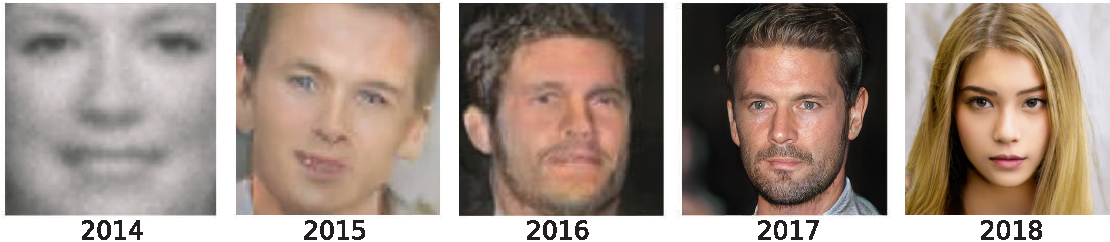
\includegraphics[width=\textwidth]{generative-evolution.pdf}
	\caption{Increasingly realistic qualities of the generated faces using generative adversarial networks as shown in \protect\cite{brundage2018malicious}; images are taken from \protect\cite{goodfellow2014gan}, \protect\cite{radford2015dcgan}, \protect\cite{liu2016cogan}, \protect\cite{karras2017pggan}, and \protect\cite{karras2019stylegan}.} 
	\label{fig:generative-evolution}
\end{figure}


Inherently, unsupervised learning is less well-defined than supervised learning, and this is the reason why unsupervised learning is sometimes synonymous with clustering, because finding clusters is usually as much an unsupervised learning system can do.
However, the recent success of deep learning introduced a new breed of generative models, enabling the end-to-end generation of complex data such as photos and audio signals.
\emph{Generative adversarial networks} (GAN) \cite{goodfellow2014gan} are the most notable among them, and their performance in generating realistic images has been improving at an extraordinary pace, as shown in Figure \ref{fig:generative-evolution}.
Combined with the various techniques for manipulating the semantic information in GANs as will be introduced in Section \ref{ch:deeplearning}.\ref{sec:gan}, this hints at completely new kinds of generative methodologies for audio processing.


In this context, this thesis aims to design and develop improved methods for automatic music transcription powered by deep generative models.
The idea specifically hypothesizes that by training a generative model, it is possible to learn disentangled representations, from which the information necessary for transcription can be easily extracted, as depicted in Figure \ref{fig:autoencoder}.
By doing so, the ultimate objective is to build an end-to-end differentiable model that connects the piano roll representation to audio signals, in order to perform automatic music transcription --- obtaining the most likely piano roll representation for given a audio waveform.


\subsection{On the Broader Context of Machine Listening in AI Research}

Using generated audio data and generative models is partly motivated by the fact that synthesized music is more prevalent and perceptually more familiar to people than synthesized texts or pictures.
Many commercial music tracks are often produced entirely using software instruments, except for the vocal parts.
This suggests that synthesized and generated audio may more accurately model the distribution of the real audio data to be transcribed.
This generative approach also aligns well with how actual musicians transcribe music, where they match given audio with their knowledge of how the instruments sound when played in a certain combination of rhythms and melodies.
Therefore it is reasonable to claim that machines should also be able to perform in a similar way, provided that a proper representation of knowledge about the music and instruments is available.

The task of automatic music transcription shares many common values with other machine learning tasks, such as image segmentation, machine translation, and speech recognition, in the sense that the core task is to build an intelligent system that can extract and process useful information conveyed in complex signals.
This is an essence of artificial intelligence (AI)
--- a system that perceives its environment and takes actions that maximizes the utility \cite{russell2009ai} --- 
where an intelligent system has to understand the semantics of complex data coming from the environment in order to perform well in its tasks.
To this end, the problem of automatic music transcription is not just an intriguing task in music technology but will also be a key component of the AI-enabled future society, constituting a musical component of the artificial general intelligence (AGI), in the form of advanced machine musicianship \cite{rowe2003musicianship}.


\subsection{Organization of The Thesis}


This thesis examines the possibility of using deep generative models to learn relevant musical concepts and inform a music transcription model to incorporate them.
There exists a rich history of research aiming at the understanding of musical sounds and automatic music transcription; to validate this claim as a feasible research direction and place this thesis in the context of this continuum of research, Chapter \ref{ch:mir} provides a review of the standard methods and the current state of the art in automatic music transcription research.
Deep learning techniques are employed as a building block throughout this thesis, and a general introduction to deep learning and deep generative models is provided in Chapter \ref{ch:deeplearning}, with a focus on generative adversarial networks.

In Chapter \ref{ch:monophonic}, we first consider a subproblem of music transcription, i.e. monophonic pitch estimation, and learn that convolutional neural networks predicting two-dimensional time-frequency representations can constitute an effective strategy, which we build and extend in the subsequent chapters.
Chapter \ref{ch:synthesis} examines the applications of deep generative models in music analysis and synthesis tasks, by introducing a WaveNet-based music synthesis model that learns a multi-dimensional timbre representation.
In Chapter \ref{ch:adversarial}, generative adversarial networks are used to apply a music language model that can help improve a piano transcription model.
In Chapter \ref{ch:timbre}, we combine the analysis and synthesis methods developed in the preceding chapters and present a multi-instrument polyphonic music transcription system.
Finally, concluding remarks are provided in Chapter \ref{ch:conclusions}.



%!TEX root = ../dissertation.tex
% this file is called up by thesis.tex
% content in this file will be fed into the main document

%: ----------------------- introduction file header -----------------------
% the code below specifies where the figures are stored
\graphicspath{{2-deeplearning/figures/}}

\chapter{Deep Learning in a Nutshell}\label{sec:deeplearning}
\label{ch:deeplearning}

Since recently, a family of machine learning research under the buzzword \emph{deep learning} has incurred many groundbreaking changes to the world of artificial intelligence, making the long-waited dream of the \emph{artificial general intelligence} (AGI) \footnote{a loosely defined term referring to human-level intelligence, i.e. an AI system that can solve complex problems in various, even previously-unseen domains with self-understanding and autonomous self-control. \cite{goertzel2007agi}} look not so distant in the future.
The impact of deep learning has been so dramatic that many successful applications of deep learning like DeepMind's AlphaGo outplaying the human Go champion and Google's neural machine translation have became familiar to the general public.
The core idea of using artificial neural networks to process complex information traces back to the earliest days of computing \cite{kleene1951representation}, but it has long been considered less effective than alternative methods, such as support vector machines or probabilistic graphical models.
Since around 2010, it has been increasingly shown that neural networks can substantially outperform those other approaches and have much more capability for further improvements, and that the lower performance of neural networks in the past was merely due to insufficient data, the lack of computational power, and some numerical tricks that have not been employed before.
This finding has opened the era of deep learning, a term coined after the fact that neural networks often employ multiple layers of learned feature transformations, and is continuing to innovate virtually all fields of science and engineering, including, of course, music technology.

This chapter reviews the essential concepts and terminologies of deep learning, from the basic architectures and techniques to the most recent advances in deep generative models.
The purpose of this chapter is to present a historical perspective toward deep generative models and to provide a motivation for building music transcription systems upon them in the proposed research.


\section{Neural Network Architectures}

The key idea of an artificial neural network in the simplest setting is to find an appropriate matrix $W$ to model the relationship between variables $\bm{x}$ and $\bm{y}$, so that
\begin{equation}\label{eqn:perceptron}
	\bm{y} = \sigma(W \bm{x})
\end{equation}
is a good approximation, where $\sigma$ is a nonlinear function like the sigmoid or the hyperbolic tangent.
This model in Equation \ref{eqn:perceptron} is also known as a \emph{perceptron} \cite{rosenblatt1957perceptron}, one of the first artificial neural networks in history.
This computation --- a matrix multiplication followed by a nonlinear activation --- can be applied multiple times, like
\begin{equation}\label{eqn:mlp}
	\bm{y} = \sigma(W_3\sigma(W_2 \sigma(W_1 \bm{x}))),
\end{equation}
which gives the model more expressive power, meaning that it can learn more complex relationship in the data that the previous model could not discern, e.g. the XOR problem \cite{riedmiller1994mlp}.
The model in Equation \ref{eqn:mlp} is called a \emph{multilayer perceptron} (MLP) in a sense that it is a concatenation of perceptrons, and the fact that it contains multiple layers is why these neural networks are called ``deep".


A multilayer perceptron is a special case of feedforward neural networks, which refer to any computational graph that does not contain a cycle.
A popular model under this category is \emph{convolutional neural networks} (CNN), which uses a convolution (a cross-correlation, to be precise) with fixed-size kernels instead of matrix multiplications.
A 2-D convolutional layer takes input arrays $X_c \in \mathbb{R}^{H \times W}$, $c \in \{ 1, \cdots, C \}$, and produces output arrays $Y_d \in \mathbb{R}^{H \times W}$, $d \in \{ 1, \cdots, D \}$.
The kernels $K_{cd} \in \mathbb{R}^{K_1 \times K_2}$, $c \in \{ 1, \cdots, C \}$, $d \in \{ 1, \cdots, D \}$, and the biases $\bm{b} \in \mathbb{R}^D$ are the parameters to be optimized, and the output is calculated as:
\begin{equation}\label{eqn:convnet}
Y_{d}[i,~j] = \sum_{m=1}^{K_1} \sum_{n=1}^{K_2} \sum_{c=1}^C K_{cd}[m,~n] X_c[i+m,~j+n] + b_d
\end{equation}
There are various options to this operation including whether to pad the input or trim the output of the convolution to according to the kernel size, and how much to stride the kernels while moving along the input arrays.
The 2-D convolution is suitable for image data, where the initial $C$ can be the 3 RGB channels of color images, while the similarly-defined 1-D and 3-D convolutions are more often used with time-series and video data respectively.

Using convolutional layers results in a fewer number of parameters to learn in each layer than the equivalent multilayer perceptron, allowing deeper models for the same total number of parameters.
LeNet \cite{lecun1995lenet} for digit classification is what pioneered the technique of using convolutional layers in neural networks, and it is an essential building block of the majority of deep learning methods, including the models that surpassed the human-level accuracy in the ImageNet Large Scale Visual Recognition Challenge (ILSVRC) \cite{krizhevsky2012imagenet, simonyan2014vgg, szegedy2015googlenet, he2016resnet}.
A standard practice of building a CNN is to stack a multiple convolutional layers along with pooling layers to obtain a compact feature repesentation, which is fed to a multi-layer perceptron as in Equation \ref{eqn:mlp} to produce output.
The layers of MLP are called fully connected or dense layers, because unlike the convolutional layers, the weight matrix used in the matrix multiplication associates every pair of the input and output features.
\emph{Fully convolutional networks}, which omit the fully connected layers that are typically placed at the last stages of neural networks, do not require a fixed input and output size and are known to perform well for image segmentation \cite{shelhamer2017fcn}.
Using the ability of deep convolutional layers extracting complex semantic information from images, many artistic applications have been developed, such as the transfer of artistic style from one image to another \cite{gatys2015style}, and a captivating transformation of images using neural network weights known as \emph{Deep Dream} \cite{mahendran2016deepdream}.


A network with cyclic connections is called a \emph{recurrent neural network} (RNN), and has been successfully applied to modeling sequence data.
Because it is hard for a recurrent neural network to propagate long-range dependencies through a chain of recurrent connections, specific recurrent units called long short-term memory (LSTM) \cite{hochreiter1997lstm} and gated recurrent unit (GRU) \cite{cho2014seq2seq} are devised to resolve the problem and are considered essential for recurrent neural networks.
A formulation of recurrent neural network called the sequence-to-sequence model \cite{cho2014seq2seq,sutskever2014seq2seq}, which can model a mapping from variable-length input to variable-length output, is well known to be very effective for machine translation, and is deployed in production in Google's translation services \cite{wu2016google}.
An important technique for building recurrent neural networks is \emph{attention} \cite{bahdanau2014attention}, which allows the network to focus on a specific part of a sequence.
The attention mechanism is shown to be effective in tasks including not only machine translation as in the original paper, but also in image description generation \cite{karpathy2017desc}, speech recognition \cite{chorowski2015speech}, and question answering \cite{sukhbaatar2015memory}.

\emph{Reinforcement learning} is a formulation of machine learning where a software agent takes actions in an environment to maximize the reward given according to the actions \cite{sutton2018reinforcement}.
This formulation is inspired by behaviorist psychology and is well-suited for environments that require explorations by the agent, such as robotics and games.
Deep Q-Network (DQN) \cite{mnih2015dqn} is a neural network model designed for reinforcement learning, which has been successfully applied to automatically playing Atari games \cite{mnih2013atari} and the agent playing the game of Go that surpassed the human level \cite{silver2016alphago}.


\section{Performance Optimization Techniques}

The success of deep learning was possible not only because of the architectural design of deeper models and the hardware capable of supporting such models, but also thanks to the numerous elaborate techniques and clever tricks that enabled previously impossible performances.

Training a neural network involves optimization of its parameters, e.g. the weights $W$ in Equation \ref{eqn:perceptron}-\ref{eqn:mlp} and the kernels $K_{cd}$ in Equation \ref{eqn:convnet}, which typically requires the gradient of the loss function, i.e. the partial derivatives with respect to all of the model's parameters.
It is feasible to manually derive the gradient for simple models, but for deep neural networks it is often too complex and error-prone to calculate the derivative by hand.
For this reason, a method called backpropagation \cite{werbos1982backpropagation, rumelhart1986backpropagation} was introduced based on the ideas of automatic differentiation \cite{linnainmaa1970ad} and revived neural network research that had been largely abandoned.
The popularization of \emph{backpropagation} in the 1980s partly contributed to the ending of the first AI winter, leading to the first commercially successful application of neural network in optical digit recognition and speech recognition.
Backpropagation is still a fundamental element of deep learning, and many deep learning frameworks are capable of automatically calculating gradients using backpropagation when a compute graph is given.
This enables the developer to write only the forward calculation and run the backpropagation automatically, greatly improving the productivity.


Once a gradient is known, the standard way of optimizing a neural network is to use a variant of \emph{stochastic gradient descent} (SGD), where the direction of the gradient descent is determined only based on a mini-batch of training data.
Although using only a tiny subset of training data makes the gradient unstable, in practice, stochastic gradient descent converges faster than batch gradient descent using the same amount of training samples.
Adding momentum in the gradient descent optimizer has shown to be effective for finding the convergence even faster, and many schemes for applying the momentum have been introduced, such as Adagrad \cite{duchi2011adagrad}, RMSprop \cite{hinton2012rmsprop}, Adadelta \cite{zeiler2012adadelta}, and Adam \cite{kingma2015adam}.
While Adam is by far the most popular choice of optimizer, a few modification to Adam's algorithm have been proposed, including Eve \cite{koushik2016eve} using feedback from the objective function, Nadam \cite{dozat2016nadam} incorporating Nesterov's accelerated gradient descent, and AMSgrad \cite{reddi2018amsgrad} fixing a failure case of Adam where it does not converge to the optimum even in a simple convex optimization problem.

Historically, the sigmoid and the hyperbolic tangent function have been popular choices for the nonlinearity, but it is surprisingly shown \cite{nair2010relu} that the \emph{rectified linear units} (ReLU),
\begin{equation}
	f(x) = \max \{ x, 0 \},
\end{equation}
generally improves the accuracy of deep learning models.
It is also known that neural networks with ReLU activations converge faster, and more robust to the vanishing gradient problem.
A number of ReLU variants, including leaky ReLU \cite{xu2015leakyrelu}, parametric ReLU (PReLU) \cite{he2015prelu}, SReLU \cite{jin2015srelu}, have been devised and shown to be effective in some cases.


As with any other machine learning methods, overfitting is a problem to overcome for deep learning models as well.
While directly adding a L1 or L2 regularization term of weights is possible, a few cleverer tricks for preventing overfitting have been devised and widely employed, and they are treated as regularization methods in a wider sense.
\emph{Dropout} \cite{srivastava2014dropout} is a simple yet powerful regularization method that turns off a random subset of activations during the training process.
Because the network has to learn how to make accurate predictions using only a random subset of its components, the training becomes more robust and less susceptible to overfitting.
\emph{Batch normalization} \cite{ioffe2015batchnorm} is a method to reduce what the covariance shift of activations, by performing normalization for each training mini-batch so that the activations of each layer have zero mean and unit variance, and is also known to improve the generalizability of the trained model.
Despite being relatively new, dropout and batch normalization are drop-in methods that can be added to most deep architectures with almost no changes to code and yet significantly improve the performance, and are thus included almost by default in the majority of newer deep models.
\emph{Scaled exponential linear units} (SELU) \cite{klambauer2017selu} use a special activation function that induces a self-normalizing property over layers, making the activations have zero mean and unit variance without using batch normalization explicitly.


Additionally, because typical neural networks contain thousands to millions of parameters to train, a proper initialization of the weights prior to training is important.
In early days of deep learning, unsupervised pre-training of weights \cite{bengio2007greedy,erhan2010pretraining} was considered necessary, but recently it is shown that a simple random initialization of weights is sufficient with the current computational power of the hardware.
A widely practiced way of initializing the weights without unsupervised pre-training is to sample from a Gaussian or uniform distribution, scaled according to the number of input and output nodes \cite{glorot2010initialization,he2015prelu}.


\section{Toward Deep Generative Models}

Statistical models that describe how data is generated are called \emph{generative models} and provide means of generating samples of data, either by directly modeling the data distribution or through a sampling procedure specified by the model which implicitly defines the probability distribution.
This is in contrast with \emph{discriminative models}, which can only predict the labels corresponding to the given data samples.

\subsection{Traditional Models}

Classic examples of generative models include \emph{na\"{i}ve Bayes classifiers} \cite{maron1961naive} which model a conditional distribution of each feature assuming they are conditionally independent given the label and use Bayes' theorem to predict the labels.
\emph{Gaussian mixture models} (GMM) \cite{everitt1981mixture} approximates the data distribution with a mixture of multivariate gaussian distributions.

While these simple models work effectively to a certain degree with a well-crafted set of features, it is desirable to have generative models that can capture more intricate geometry of the data distribution.
\emph{Probabilistic graphical models} (PGM) specify the structural dependencies between random variables using graphs, with nodes representing random variables and connections between them representing their dependencies.
The graphs can have directed or undirected connections to formulate the joint probability distributions of the variables.
\emph{Hidden Markov models} (HMM) \cite{rabiner1989hmm} and \emph{latent Dirichlet allocation} (LDA) \cite{blei2003lda} are special cases of directed probabilistic graphical models, also called \emph{Bayesian networks}, and are widely used for sequence modeling and topic modeling, respectively.
Undirected graphical models are also called \emph{Markov random fields} (MRF), and have many applications in image processing, typically by having connections between nodes corresponding to adjacent pixels.
Undirected graphical models where every pair of nodes has a connection are called \emph{Boltzmann machines} and are capable of learning internal representations of data.

\subsection{Early Deep Generative Models and Autoregressive Models}

\emph{Restricted Boltzmann machines} (RBM) are simplified variants of Boltzmann machines consisting of two layers of nodes with only interlayer connections, and unlike Boltzmann machines, there exists a relatively efficient algorithm \cite{hinton2005cd} for training restricted Boltzmann machines.
\emph{Deep belief networks} (DBN) \cite{hinton2006dbn} are composed of multiple layers of restricted Boltzmann machines, which can be trained using greedy layer-wise optimization, and are capable of classifying hand-written digits as well as conditionally generating them.
Although deep belief networks are one of the first successful deep learning applications and gave many architectural and algorithmic insights to the development of deep learning in the subsequent years, the algorithms for training DBNs are not as scalable as those for other discriminative models like stochastic gradient descent, and eventually faded away in favor of the discriminative models that runs more effectively with a larger scale of data.

An alternative method to generate data samples using a neural network is to produce one element (i.e. one audio sample or one pixel) at a time by feeding the previous elements to the network.
This approach is called an autoregressive model, and many architectures based on this idea including NADE \cite{larochelle2011nade}, DARN \cite{gregor2013darn}, RIDE \cite{theis2015ride}, DRAW \cite{gregor2015draw}, PixelCNN/PixelRNN \cite{oord2016pixel}, SampleRNN \cite{mehri2016samplernn}, WaveNet \cite{oord2016wavenet}, and WaveRNN \cite{kalchbrenner2018wavernn} are proposed and shown to be capable of generating image and audio samples.
However, in addition to being inevitably slow having to repetitively run the model for every element, a drawback of autoregressive models is the difficulty of interpreting the representation, because the autoregressive model only encodes the local dependency of one sample on the adjacent elements and does not provide a compact latent representation corresponding to the global structure.

\subsection{Variational Autoencoders}

A straightforward method to obtain a compact latent representation from unlabeled data is to build an encoder that transforms the input data into a smaller latent dimension, followed by a decoder that maps it back to the original data.
This architecture is called an \emph{autoencoder} \cite{bengio2009deeplearning}, and being a deep extension to principal component analysis (PCA), it is capable of learning a nonlinear mapping for dimensionality reduction.
The autoencoder architecture are shown to be effective at encoding the latent representation of data, through a few successful variants including sparse autoencoder \cite{ng2011sparse} which produces a sparse representation of the input data, denoising autoencoder \cite{vincent2008denoising} which is capable of reducing noise or recover a redacted portion of an image, and contractive autoencoder \cite{rifai2011contractive} which adds a regularization term to make the model robust to slight variations of input values.


Autoencoders are not generative models in a strict sense, because, while its decoder part can produce data samples from their latent representations, it lacks the ability to randomly sample the points in the latent dimensions that corresponds to the data distribution.
\emph{Variational autoencoders} (VAE) \cite{kingma2013vae} fix this problem by restricting the posterior latent distribution to be Gaussian.
This is achieved by variational inference, reformulating the evidence lower bound (ELBO) of the data log-likelihood as:
\begin{equation}\label{eqn:vae}
\log p(\bm{x}) \ge \mathcal{L}(p_\theta, q_\phi) = \mathbb{E}_{q_\phi(\bm{z}|\bm{x})} [\log p_\theta(\bm{x}|\bm{z})] - \mathrm{KL}(q_\phi(\bm{z}|\bm{x}) || p(\bm{z})),
\end{equation}
where $q_\phi(\bm{z}|\bm{x})$ models the encoder and $p_\theta(\bm{x}|\bm{z})$ models the decoder, and both are parameterized using neural networks which provides a flexible and differentiable family of functions.
Note that maximizing $\mathcal{L}$ will maximize the first term of RHS, the log likelihood of the reconstructed data, and minimize the second term, the KL divergence between the encoded data distribution and the prior, serving as a regularizer that induces the posterior to be Gaussian.
The Gaussian prior gives the KL divergence a closed-form solution making it straightfoward to derive the derivative according to $\phi$, whereas the first term contains an expectation over a distribution depending on $\phi$, which disallows moving the gradient operator into the expectation and makes the stochastic gradient descent and backpropagation impossible.
A reparameterization trick is used to address this issue, by setting $\bm{z} = g({\epsilon}, \bm{x}) = \bm{\mu}_\phi (\bm{x}) + {\epsilon} \cdot \bm{\sigma}_\phi(\bm{x})$ where $\epsilon \sim \mathcal{N}(0, 1)$, which gives:
\begin{equation}\label{eqn:reparam}
\nabla_\phi \mathbb{E}_{q_\phi(\bm{z}|\bm{x})} [\log p_\theta(\bm{x}|\bm{z})] = \nabla_\phi \mathbb{E}_{\epsilon} [\log p_\theta(\bm{x}|g(\epsilon, \bm{x}))] = 
\mathbb{E}_{\epsilon} [\nabla_\phi \log p_\theta(\bm{x}|g(\epsilon, \bm{x}))],
\end{equation}
making the stochastic gradient ascent and backpropagation on the ELBO possible.


The biggest drawback of variational autoencoders, however, is the blurriness in reconstructed images, that may come from the inexactness of the Gaussian assumption and the variational lower bound used by the model \cite{doersch2016tutorial}.
There have been many attempts to overcome this by allowing more flexible prior distributions \cite{rezende2015flow} as well as better latent representations \cite{kingma2016iaf}.
VQ-VAE \cite{oord2017vqvae} uses discrete prior and posterior distributions, and is able to generate less blurry images and perform speaker conversion using raw audio.
Variational autoencoders are powerful deep generative models with the advantages of having a single objective function to be optimized and thus having a stable training scheme.
Despite being one of the most successful types of deep generative models to date, it remains to be seen if variational autoencoders can be extended to become a building block of an automatic music transcription system.


\section{Generative Adversarial Networks}\label{sec:gan}

\emph{Generative adversarial networks} (GAN) \cite{goodfellow2014gan} are a family of deep generative models that have become extremely popular.
Unlike other deep neural network models that use optimization to find the weights minimizing the loss function, GANs try to find a Nash equilibrium between its two components, the generator and discriminator.
Given the training data $\bm{x}\sim p_{\mathrm{data}}$ and the prior of latent vectors $\bm{z} \sim p_{\bm{z}}$ which typically is a multivariate Gaussian distribution, GAN performs the following minimax game:
\begin{equation}\label{eqn:gan}
	\min_{G} \max_{D} \Big[ \mathbb{E}_{\bm{x} \sim p_{\mathrm{data}}} {\log D(\bm{x})} + \mathbb{E}_{\bm{z} \sim p_z} \log \left ( 1 - D(G(\bm{z})) \right ) \Big],
\end{equation}
where the generator $G$ learns to transform a noise vector $\bm{z}$ into a data point that can fool the discriminator as if it is a real data sample, while the discriminator $D$ tries to correctly distinguish the output of generator $G(\bm{z})$ from the real data $\bm{x}$.
Because the second expectation has a near-zero gradient where $D(G(\bm{z})) \approx 0$, i.e. the discriminator classifies the generated samples as fake, the authors suggests using a non-saturating loss for training the generator:
\begin{equation}\label{eqn:nsgan}
\max_{G} \mathbb{E}_{\bm{z} \sim p_{\bm{z}}} \log D(G(\bm{z})),
\end{equation}
which maximizes the log-likelihood of the discriminator classifying the generated samples as real.


\subsection{Evolution of the GAN Architecture}

The original formulation of GAN uses neural networks, which can only be applied to simple datasets of up to 32$\times$32 images such as MNIST, CIFAR-10, and Toronto Face Dataset.
LAPGAN \cite{denton2015lapgan} is the first GAN formulation to generate 64$\times$64 images, which builds upon a Laplacian pyramid of convolutional layers that conditionally generates an image that is twice larger, gradually building 64$\times$64 images from 4$\times$4 samples.
DCGAN \cite{radford2015dcgan} provides a simpler method of training convolutional GANs by following a list of architectural choices, making adversarial training of 64$\times$64 images possible only using one generator and one discriminator.
Together with Improved GAN \cite{salimans2016improved} which proposed now-standard tricks such as feature matching, minibatch discrimination, historical averaging, and one-sided label smoothing to generate 128$\times$128 images, the DCGAN architecture is employed by virtually all subsequent GAN applications.
For photo-realistic images synthesis in a higher resolution, StackGAN \cite{zhang2017stackgan2} uses a multi-stage GAN architecture to synthesize 256$\times$256 images, and progressive growing of GANs \cite{karras2017pggan} uses a training scheme that gradually switches to larger GANs to generated photo-realistic images of size 1024$\times$1024.
The GAN architecture is also applicable to 3-D \cite{wu2016gan} and 1-D \cite{donahue2018wavegan} synthesis.


\subsection{The GAN Zoo}

GANs are notoriously difficult to train \cite{arjovsky2017principled}; its convergence is unstable because of the minimax nature of its formulation, and the generator network may simply memorize and output just a few samples of training data, an undesirable phenomena called mode collapsing.
A plethora of variations of GAN have been proposed to mitigate this problem, aiming to stabilize the training and/or improve the perceptual quality of generated samples.
A common approach among them is to devise a different loss function or to add a regularization term to the loss function that penalizes mode collapsing.

$f$-GAN \cite{nowozin2016fgan} is a generalization of the original GAN using a family of $f$-divergences in addition to the original GAN's formulation using Jensen-Shannon divergence.
Wasserstein GAN (WGAN) \cite{arjovsky2017wgan} minimizes the Wasserstein distance between the model and real distribution, and was later extended to WGAN-GP \cite{gulrajani2017wgan} which uses a gradient penalty that does not require weight clipping as in Wasserstein GAN.
Based on WGAN's observation that Lipschitz continuity of GAN is beneficial, spectral normalization \cite{miyato2018spectral} is another technique to impose Lipschitz continuity that is more stable and provides higher diversity in generated images than gradient penalty.
Wasserstein distance is not an $f$-divergence but a special case of integral probability metrics (IPM), which also includes maximum mean discrepancy (MMD) distance, on which MMD GAN \cite{li2017mmdgan} and Distributional Adversarial Networks (DAN) \cite{li2017dan} are based.
Fisher GAN \cite{mroueh2017fishergan} and Sobolev GAN \cite{mroueh2018gan} are also IPM-based GAN models.

Least-Square GAN (LSGAN) \cite{mao2017lsgan} uses least-square losses instead, and also can be trained with gradient penalty \cite{mao2017effectiveness} which achieves a training stability similar to WGAN-GP's.
Energy-Based GAN (EBGAN) \cite{zhao2017ebgan} views the discriminator as an energy function that puts low energy near the data manifold, and uses an autoencoder to model the discriminator. Boundary Equilibrium GAN (BEGAN) \cite{berthelot2017began} extends the EBGAN architecture using Wasserstein distance to balance the generator and discriminator during training.
CoulombGAN \cite{unterthiner2017coulomb} formulates the GAN setup in terms of a potential field of charged particles, and DRAGAN \cite{kodali2017gan} poses GAN training as a regret minimization problem in online learning.
Unrolled GAN \cite{metz2016unrolled} uses a surrogate objective function for the more stable generator updates, which approximates the optimal discriminator in the generator's perspective.
While there are many more GAN formulations claiming to be superior than others, a large-scale empirical study \cite{lucic2017gan} suggested that the none of the popular variants actually outperforms the original GAN, provided that the hyperparameters are sufficiently optimized.


\subsection{Conditional Generation}

It is usually desirable to generate samples according to certain conditions, e.g. generating images for a specific digit.
Conditional GAN (cGAN) \cite{mirza2014conditional} is an architecture where the generator can use the class label as well as the noise input to produce samples.
Auxiliary Classifier GAN (AC-GAN) \cite{odena2016acgan} is an extension to cGAN in which the discriminator can also serve as a classifier.
InfoGAN \cite{chen2016infogan} can perform conditional generation in a completely unsupervised manner, i.e. without using class labels during training, by maximizing the mutual information between a subset of the latent variables and the observations.

sAll of the above architectures use conditional latent components concatenated to the other feature components, which makes training a conditional GAN with a large number of classes difficult.
\cite{miyato2018cgan} overcomes this by performing projections on the feature space of the discriminator, successfully demonstrating conditional image synthesis on the 1,000 classes of images of the ILSVRC dataset \cite{russakovsky2015imagenet}.


\subsection{GANs with Encoder}

While the generator can produce data samples from latent vectors, the default GAN formulation does not provide means to obtain the latent vector corresponding to the given data sample.
This task is usually referred to as inference in GAN literature, and many architectures have been proposed to achieve this.
Adversarially learned inference (ALI) \cite{dumoulin2017ali} and Bidirectional GAN (BiGAN) \cite{donahue2016bigan} both refers to the same architecture that jointly trains an encoder that calculates the inverse of generator, by training discriminator to operate on pairs of the data samples and the corresponding latent vectors:
\begin{equation}\label{eqn:bigan}
\min_{G,~E} \max_{D} \Big[ \mathbb{E}_{\bm{x} \sim p_{\mathrm{data}}} {\log D(E(\bm{x}), \bm{x})} + \mathbb{E}_{\bm{z} \sim p_{\bm{z}}} \log \left ( 1 - D(z, G(\bm{z})) \right ) \Big].
\end{equation}

ALICE \cite{li2017alice} resolves the non-identifiability problem present in ALI that , by adding a conditional entropy regularization term, and bidirectional conditional GAN (BCGAN) \cite{jaiswal2017bcgan} combines BiGAN with cGAN to perform both inference and conditional synthesis.
Mode regularized GAN (MRGAN) \cite{che2016mrgan} has a similar setup of jointly training an encoder network and uses a regularization term on the generator loss that discourages mode collapse:
\begin{equation}\label{eqn:mrgan}
\min_{G,~E} \Big[ - \mathbb{E}_{\bm{z} \sim p_{\bm{z}}} [ \log  D(G(\bm{z})) ]
+ \mathbb{E}_{\bm{x} \sim p_{\mathrm{data}}} [ \lambda_1 d(x, G(E(\bm{x}))) + \lambda_2 \log D(G(E(\bm{x}))) ] \Big],
\end{equation}
where $d$ is a distance metric defined in the data space.
Adversarial generator-encoder (AGE) networks \cite{ulyanov2017age} achieve a comparable quality to other GANs using only two components, the generator and the encoder, without the discriminator.


\subsection{Fusing GAN with Variational Autoencoder}

The idea of combining the autoencoder architecture and adversarial training gave birth to new kinds of deep generative models.
Adversarial Autoencoders (AAE) \cite{makhzani2015aae} jointly train a standard autoencoder and an adversarial network that regularizes the posterior distribution to be Gaussian.
VAE-GAN \cite{larsen2015vaegan} trains a concatenation of VAE and GAN using the sum of their loss functions, and Adversarial Variational Bayes (AVB) \cite{mescheder2017adversarial} similarly extends on variational autoencoder using an auxiliary discriminator network to perform adversarial training, which brings the variational lower bound tighter to the maximum likelihood.
$\alpha$-GAN \cite{rosca2017alphagan} is yet another method to combine the VAE and GAN loss, which adds additional discriminator on the $\bm{z}$ domain to distinguish the encoded data samples from the Gaussian prior.


\subsection{Appilcations of GAN}

Many image-to-image translation models have been developed using GANs. Pix2pix \cite{isola2016pix2pix} is trained on pairs of cross-domain images, and learns to translate images between the domains, e.g. satellite images to corresponding maps, day photos to night photos, and edges of images to the original.
DiscoGAN and CycleGAN \cite{kim2017discogan, zhu2017cyclegan} are capable of performing similar tasks, but does not require paired training samples, greatly expanding the ranges of datasets that can be used for training.
StarGAN \cite{choi2017stargan} learns to translate between more than two domains.

GAN has been successfully applied to many other tasks, including image super-resolution (AffGAN) \cite{sonderby2016amortised}, text-to-image synthesis (StackGAN) \cite{zhang2017stackgan,zhang2017stackgan2}, text generation (Boundary-seeking GAN, BGAN) \cite{hjelm2018bsgan}, and speech enhancement (SEGAN) \cite{pascual2017segan}.


\subsection{Evaluation of Generated Samples}

Unlike discriminative models that can be evaluated using well-defined metrics, it is not as straightforward to evaluate the performance of generative models.
Structural similarity (SSIM) \cite{wang2004ssim} and its multi-scale extension MS-SSIM \cite{wang2003msssim} can measure the similarity between two images using luminance, contrast, and structure information, and are commonly used for measuring intra-class diversity \cite{odena2016acgan}.
This metric can be useful for assessing the mode collapsing problem, but is less useful if the dataset is already diverse \cite{fedus2018equilibrium}.

Another popular method for evaluating the perceptual quality of generated images is the Inception score \cite{salimans2016improved}, based on the image classification model under the same name \cite{szegedy2015inception} which is a 1000-class image classifier trained on the ILSVRC dataset \cite{russakovsky2015imagenet}.
Assuming that meaningful images would have a low-entropy conditional label distribution, and a diverse set of generated images would have a high-entropy marginal label distribution, the Inception score can be obtained by feeding generated images to the Inception classifier and calculating:
\begin{equation}\label{eqn:inception}
\exp \left ( \mathbb{E}_{\bm{x}} \Big[ \textrm{KL} \left ( p(y|\bm{x}) || p(y) \right ) \Big] \right ).
\end{equation}
For the domains other than natural images, Inception score can be calculated using a different classifier; in \cite{donahue2018wavegan} for example, an Inception score using an audio classifier is used to evaluate the quality of generated audio excerpts.
While Inception scores correlate well with human perception, a drawback of is that the distribution of real data is not considered in the calculation, for a metric measuring how realistic the generated samples are.

Fréchet Inception distance (FID) \cite{heusel2017ttur} address this problem and provides a distance metric between the data distribution and model distribution.
FID is defined using the activations of a coding layer of the Inception-v3 model, \texttt{pool\_3} to be specific, as the Fréchet distance between multivariate Gaussian approximations of the two distributions:
\begin{equation}\label{eqn:fid}
d^2 = \left \lVert \bm{\mu}_1 - \bm{\mu}_2 \right \rVert^2 + \mathrm{Tr} \left ( C_1 + C_2 - 2 ( C_1 C_2 )^{1/2} \right ),
\end{equation}
where $\bm{\mu}_i$ and $C_i$ are the mean vector and the covariance matrix of the coding layer for each distribution.

\subsection{Theories on GAN Convergence}

\TODO{review:}

\cite{arjovsky2017principled}, \cite{kodali2017gan}, \cite{nagarajan2017local}, \cite{daskalakis2018gan}, \cite{mohamed2016implicit}, \cite{fedus2018equilibrium}, \cite{arora2017gan,arora2018gan}, \cite{mescheder2017gan,mescheder2018convergence}

\section{Summary}

\TODO{summarize}

%!TEX root = ../dissertation.tex
% this file is called up by thesis.tex
% content in this file will be fed into the main document

%: ----------------------- introduction file header -----------------------
% the code below specifies where the figures are stored
\graphicspath{{3-mir/figures/}}

\chapter{Music Information Retrieval for Transcription}
\label{ch:mir}

Being able to accurately identify all musical events from audio and transcribe them into musical notations is an essential skill for musicians as well as a paramount goal of music machine learning research.
Enabling an automatic conversion between musical audio and symbolic notations, automatic music transcription opens up many new possibilities.
The most straightforward application of automatic music transcription would be a software tool that transcribes audio recording and produces a musical score, which can aid musicians in various situations.
Automatic music transcription can help build a melody database to be used for music retrieval systems, such as query by humming \cite{molina2014humming}, where it is often very hard to obtain annotated data even when the audio files are abundantly available.
Similarly, by building a database containing symbolic information of music, music recommender systems can leverage the database to infer how much individual users would prefer the music, based on melodic, harmonic, and instrumental information present in the transcription.


As previously stated, due to the complexity and difficulty of creating a completely end-to-end music transcription system, many existing approaches focus on a specific subtask of the problem \cite{casey2008mir}, e.g. extracting onsets and beats, recognizing timbre and instruments, tracking monophonic and polyphonic pitches, or separating audio sources from a mixture.
Each of these subtasks poses interesting goals and applications even without the lofty goal of end-to-end music transcription, and they are often classified under the umbrella term of \emph{music information retrieval} (MIR).
Although this term has existed since 1960s \cite{kassler1966mir}, it was only after the late 1990s when active research on this area has spun off from computer music and computational musicology literature.
During the last two decades, numerous sophisticated and novel approaches for each of these subproblems have been introduced, that have continuously improved the performance in terms of the accuracy in predicting the correct annotations.
This chapter starts by introducing the standard pipeline of music information retrieval that are commonly employed in most MIR models and reviews the state-of-the-art techniques in each area relevant to music transcription.
The purpose of this chapter is not to provide an all-encompassing survey over the history of MIR research but to show a clear common pattern over the areas of MIR where the machine learning models have been evolving from simple heuristics based on hand-crafted features to sophisticated deep learning models with millions of parameters.
Together with the fast progress of the research on deep generative models as shown in the previous chapter, the content of this chapter provides justification and motivation for pursuing research on deep generative models for music transcription, which generally requires more sophisticated statistical models and therefore more powerful hardware than the discriminative counterpart.


\section{The Standard Pipeline}

Audio data is huge in volume; a typical audio track contains 44,100 real-numbered samples per second, and sometimes even more.
Therefore, computational methods for extracting musical information from audio usually contains a pipeline of feature extraction stages to reduce the volume and increase the interpretability of input data, as shown in Figure \ref{fig:pipeline}.
The pipeline includes a few techniques widely used in speech processing, as well as many feature extraction stages created for music-specific purposes.

\begin{figure}[t]
	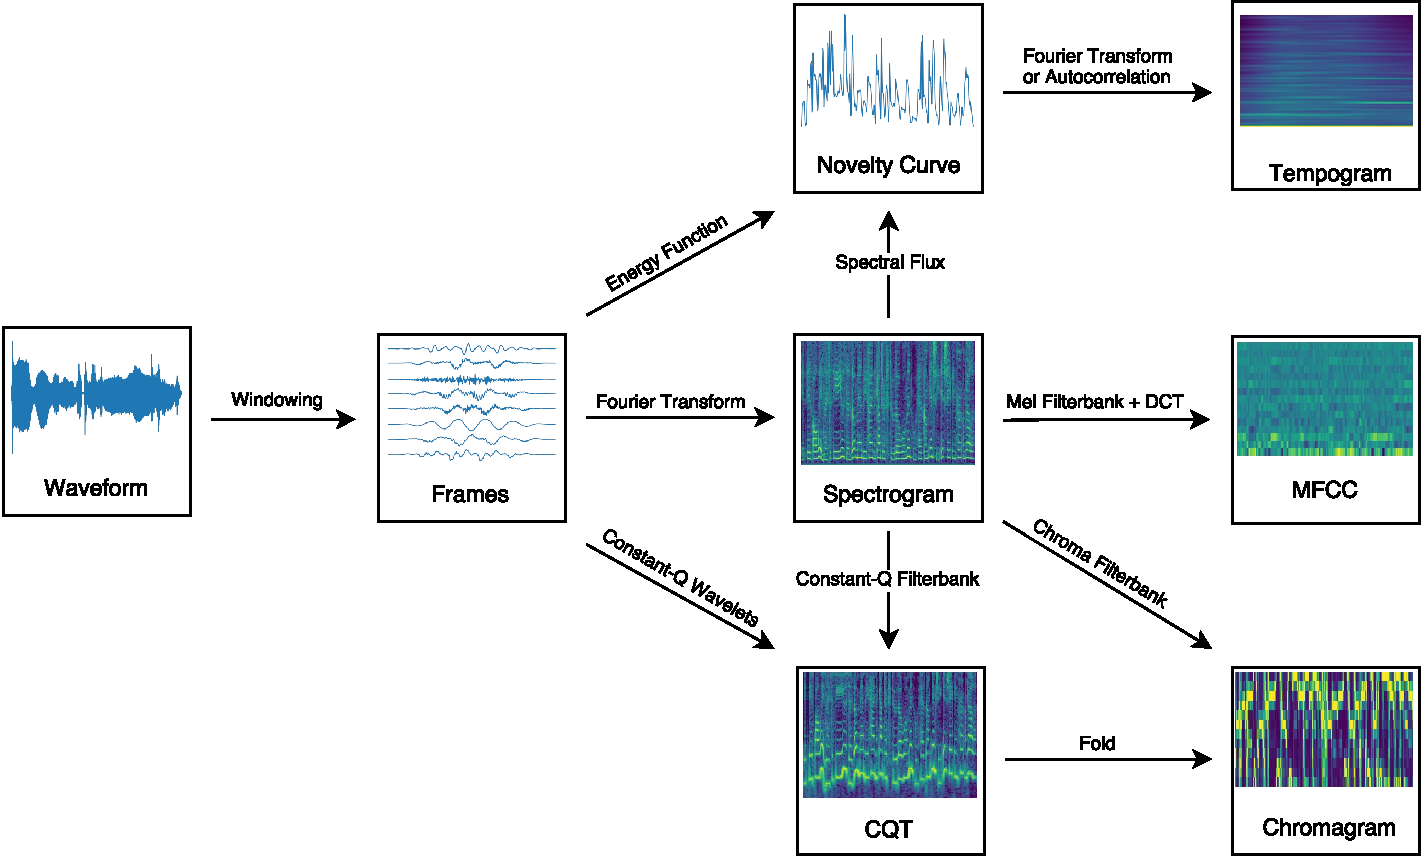
\includegraphics[width=\textwidth]{pipeline.pdf}
	\caption{\small The standard pipeline for music feature extraction. An appropriate set of feature extraction methods needs to be heuristically selected depending on the task.}\label{fig:pipeline}
\end{figure}

While there are many MIR tasks that operate on the track level, such as music recommendation, tagging, and genre classification, most subtasks of music transcription involve the prediction of labels that are dependent on time, operating either in the sample-level or frame-level.
Frames are created by taking a series of overlapping short-time audio segments, where the length of a segment typically ranges from 10 to 50 milliseconds, and optionally multiplying them by a windowing function.
Taking discrete Fourier transforms on the frames produces a \emph{short-time Fourier transform} (STFT), and the magnitude of an STFT gives a \emph{spectrogram}.
Spectrograms give very rich information about the audio; for example, the contour of melodies and the dynamics of music are usually identifiable from the spectrogram image.
Spectrograms are expressive enough to be used as an output of sound synthesis or a source separation algorithm, and the corresponding audio signals can be reconstructed without incurring significant perceptual inconsistencies \cite{griffin1984lim, leroux2010spectrogram}.
However, the dimensionality of a spectrogram is still quite high, making it computationally prohibitive to run many algorithms directly on an STFT or a spectrogram.
This necessitated further transformations by the means of filterbanks, such as \emph{Mel-Frequency Cepstral Coefficients} (MFCC) \cite{logan2000mfcc} by applying the Mel filterbank which is inspired by the human auditory perception.
\emph{Constant-Q transform} (CQT) \cite{schorkhuber2010cqt} uses a filterbank where the center frequencies of filters have a constant Q factor, which is the ratio between the center frequency and the 3 dB bandwidth of a filter.
By configuring CQT to produce 12 filters per octave, it is possible to obtain the coefficients corresponding to each musical tone, and to fold the representation to produce a \emph{chromagram} \cite{bello2005chromagram}.
To extract the beat and tempo information, a heuristic function, such as the first-order difference of the time-domain log energy function or the \emph{spectral flux} that measures the total energy increase over the STFT frequency bins, is applied to formulate a novelty curve, which measures energy bursts typically present in the onsets of notes \cite{bello2005onset}.
The onset information can then be further processed to obtain tempo information via \emph{tempogram} \cite{cemgil2000tempogram} or cyclic tempogram \cite{grosche2010tempogram}.


Once an appropriate set of features are obtained, the next steps for MIR algorithms typically involve applying a classification model.
Examples include Random forests, support vector machines (SVM), and Gaussian mixture model (GMM) classifiers that have been applied to music tagging \cite{ness2009tag}, melody extraction \cite{bittner2015contour}, and genre classification \cite{tzanetakis2002genre} tasks.
Hidden Markov models (HMM) are widely employed for modeling sequence data such as chord progressions \cite{cho2010chord} as well as to smooth the sequence output as a post-processing step \cite{khadkevich2009hmm}, often paired with Gaussian mixture models as the emission probability distribution.
Since finding a better feature representation played a crucial role in earlier MIR systems, many approaches focused on engineering sophisticated feature transformations \cite{harte2006tonnetz} and devising clever pre- and post-processing steps \cite{oudre2009chord}.


More recent approaches have successfully eliminated some or all feature transformation stages in the standard MIR pipeline by training a deep model to learn the feature from the spectrogram or audio waveforms.
Applications of deep learning arose in virtually all types of MIR tasks, including melody extraction \cite{bittner2017deepsalience}, beat tracking \cite{vogl2017drum}, and genre classification \cite{oramas2017genre}.
Apart from a small number of end-to-end approaches, most deep learning models for music still rely on predefined feature transforms such as STFT or CQT, because those features make it easier for a model to learn meaningful concepts without overfitting, using a smaller amount of parameters and thus using less powerful hardware.
In theory, however, any feature extraction stage induces a loss of information, and it suggests that the best-performing model would benefit most from the raw audio data.


\section{Multiple Fundamental Frequency Estimation}

Among the aforementioned subtasks of automatic music transcription, estimating the pitch from polyphonic recording poses the most difficult challenges, as apparent from the recent stream of results from MIREX challenges \cite{downie2014mirex}.
The task is commonly referred to as \emph{multiple fundamental frequency estimation} (Multi-F0 estimation, or MFFE) and is in some sense a superset of the onset and beat detection problems as well as chord and melody tracking problems,
since the frequency tracking task has to indicate the onset and offset of every sound, and tracking chords and melodies becomes much easier when the correct annotations for all pitch contours are available.

Many early methods for MFFE \cite{klapuri2003multiple} focused on extracting features like harmonicity and spectral smoothness from the audio spectrogram and devising a good heuristic for frequency estimation.
Another major technique for polyphonic music transcription is \emph{non-negative matrix factorization} (NMF) \cite{lee2001nmf}, based on the assumption that the spectrogram is a low-rank matrix which is a multiplication of the harmonic profile of each notes and the note activation patterns.
While some approaches \cite{gao2017nmf} based on NMF performs close to the state of the art, it has a drawback of having to obtain duplicate pitch templates for multiple instruments.
Other data-driven approaches are based on dynamic Bayesian networks \cite{raczynski2013dynamic}, hierarchical graphical models \cite{pesek2017hierarchical}, convolutional neural networks \cite{bittner2017deepsalience}, recurrent neural networks \cite{bock2012rnn,sigtia2016endtoend}, and most recently an architecture combining convolutional and bidirectional recurrent neural networks \cite{hawthorne2018piano}.

With the state of the art nearing the perfect accuracies \cite{ewert2017transcription} on the MAPS dataset \cite{emiya2010multipitch} which have been the standard evaluation dataset for piano transcription algorithms, more systematic assessments of transcription models have recently been proposed.
These include the study of invariance under data augmentation \cite{thickstun2017invariances} and the entanglement of note representations that may prevent accurate predictions for unseen combinations of notes \cite{kelz2017entanglement}.

In \cite{li2017infinite}, the idea of using on-the-fly synthesized training dataset for piano transcription was explored, using a simple fully-connected neural network operating on the CQT representation.
The idea of using generative models to predict multiple fundamental frequencies is also not new \cite{dubois2005harmonic,cemgil2006generative}, but they relied on manually designed generative models for sound generation, which might have led to poor generalizability.
Using deep generative models is expected to help overcoming this limitation, since deep learning methods is known to be excellent in learning embeddings and manifolds that are generalizable to different tasks and domains.


\section{Music Synthesis and Translation Models}

While sound synthesis is a topic that has a long history \cite{cook2002synthesis}, recent deep generative have been very successful in synthesizing breathtakingly high-quality audio signals.
We would want the synthesized music and audio signals to capture the long-term dependencies such as beats, measures, and chord progressions that ranges up to a few seconds, while the raw audio signals typically have the order of 10 thousand sameples per second.
This made end-to-end synthesis models more difficult to train than image synthesis and translation models which it usually suffices to capture dependencies ranging a few hundred pixels.
SampleRNN \cite{mehri2016samplernn}, previously discussed in Chapter \ref{ch:deeplearning} in the context of deep autoregressive models, is one of the first successful deep generative models for audio and formed a basis for the techniques used by Lyrebird, an AI startup founded by University of Montr\'{e}al students that provides API for synthesized voice of a specific person, e.g. Barack Obama.
WaveNet \cite{oord2016wavenet}, developed by Google DeepMind, uses a causal architecture using dilated convolutions to generate time-domain audio samples, and is able to produce realistic human voices and piano sounds.
WaveNet learns acoustically meaningful representations including pitch and spectral features \cite{hua2018wavenet}.
There also exist faster approaches using recurrent neural networks to produce vocal and musical audio, as found in \cite{nayebi2015gruv} and \cite{kalingeri2016generation}, albeit with lower quality when compared to WaveNet.
Tacotron \cite{wang2017tacotron, shen2018tacotron} is a fully end-to-end speech synthesizer that works directly on a sequence of characters, which can learn the pronunciation of unseen complex words and different ways of reading the same word according to the phrase semantics and punctuations.
A newer RNN-based model called WaveRNN \cite{kalchbrenner2018wavernn} is capable of generating audio that matches WaveNet in quality, yet with an enough efficiency to be able to run real-time on GPUs or even on mobile phones.
A singing synthesis model \cite{blaauw2017singing} based on the WaveNet architecture is also capable of synthesizing voice parametrically, separating the influence of pitch and timbre in the model.
A music synthesis technique employing a similar approach as the above will be a key component of the overall architecture, allowing the transcription model to generate realistic-sounding music to compare with the input audio.


Audio translation problems concern mapping input audio to a corresponding output with some desired properties, such as speech with reduced noise, singing voice separated from music, or the same speech in the voice of a different speaker.
The \emph{U-Net} architecture \cite{ronneberger2015unet} uses an encoder-decoder framework with skip connections between the hidden layers at the same level of abstraction to perform image translation, and a singing voice separation model can be trained using this architecture \cite{jansson2017separation}.
The encoder-decoder architecture with skip connections can also be trained with GAN objectives, and a few audio translation models working on spectrograms have been developed; examples include singing voice separation \cite{fan2017svsgan, stoller2017separation}, source separation \cite{subakan2017gan}, and speech enhancement \cite{pascual2017segan, donahue2017segan}.

A problem of producing spectrograms as an output of image translation model is that reconstructing the resulting audio requires the phase information.
While using the phases from the input STFT can produce acceptable results for a translation model, a phase reconstruction algorithm is required for a generative model for audio.
A GAN architecture using one-dimensional convolutions called \emph{WaveGAN} was recently introduced \cite{donahue2018wavegan}, which is capable of generating 1-second audio segments from the latent representations.
The 1-D output does not require phase reconstruction, and it was able to achieve a better perceptual quality than the audio reconstructed using 2-D GANs.
As shown in the paper, training of 1-D GANs is much more susceptible to the choice of the GAN objective than the 2-D GANs, and training GAN for longer audio sequences and extending it as a tool for disentanglement of latent semantic information or a conditional audio synthesis framework remains as a challenge.

\section{Symbolic Music Processing and Music Language Models}

Symbolic music processing refers to the techniques for processing music at a symbolic level, such as in the form of sheet music, MIDI signals, or piano roll representations.
Problems in this domain includes optical music recognition \cite{rebelo2012omr}, algorithmic composition \cite{fernandez2013ai}, and computational music theory \cite{hamanaka2013computational}, while the subject most relevant to music transcription research would be \emph{music language models}.
A music language model refers to a statistical model, often being a generative model, that encodes music theoretic knowledge to describe the structural composition and arrangement of musical elements \cite{patel2010musiclanguage}, similarly to how computational linguists build language models to describe the structure of natural languages.
A well-designed music language model can be an important component for a generative model for music, because it can serve as a prior for latent representations and can be combined with conditional synthesis models or software instruments to produce audio.

The first systematic approach of applying a linguistic theory to music was the \emph{generative theory of tonal music} \cite{lerdahl1983gttm}, which was inspired by Noam Chomsky's generative grammar \cite{chomsky1966generative} and was influential in music theory, music psychology, and cognitive musicology.
The history of algorithmic composition techniques is decades-long \cite{fernandez2013ai}, while many are artistic approaches rather than optimization problems to build a generative music language model that best approximates the real world music.
Computational methods for building music language models often include applying statistical natural language processing techniques to music, such as a recurrent neural network to build a music language models \cite{sigtia2014lm}.
The latest approaches to generate realistic sound music sequences in the symbolic domain include an application of variational autoencoder \cite{teng2017generating,tikhonov2017generation}, and a generative adversarial network \cite{yang2017midinet}.

\section{Summary}
%!TEX root = ../dissertation.tex

\graphicspath{{4-methods/figures/}}
\chapter{Methodology and Challenges}
\label{ch:methods}

The chapter outlines the prospective methodologies for this thesis and discusses the expected challenges in the proposed research directions.
It is unavoidable that the content of this chapter includes a certain degree of abstractness and ambiguity, because, as in most machine learning research, there is no predefined protocol for performing the research, and the very goal of this study lies on finding a methodology that works.
In light of this, the following section illustrates the high-level ideas, and the perspectives on generative models and the concept of disentanglement are presented, followed by the description of the evaluation metrics and the datasets to be used in the research.


\section{The High-Level Ideas}

\begin{figure}
	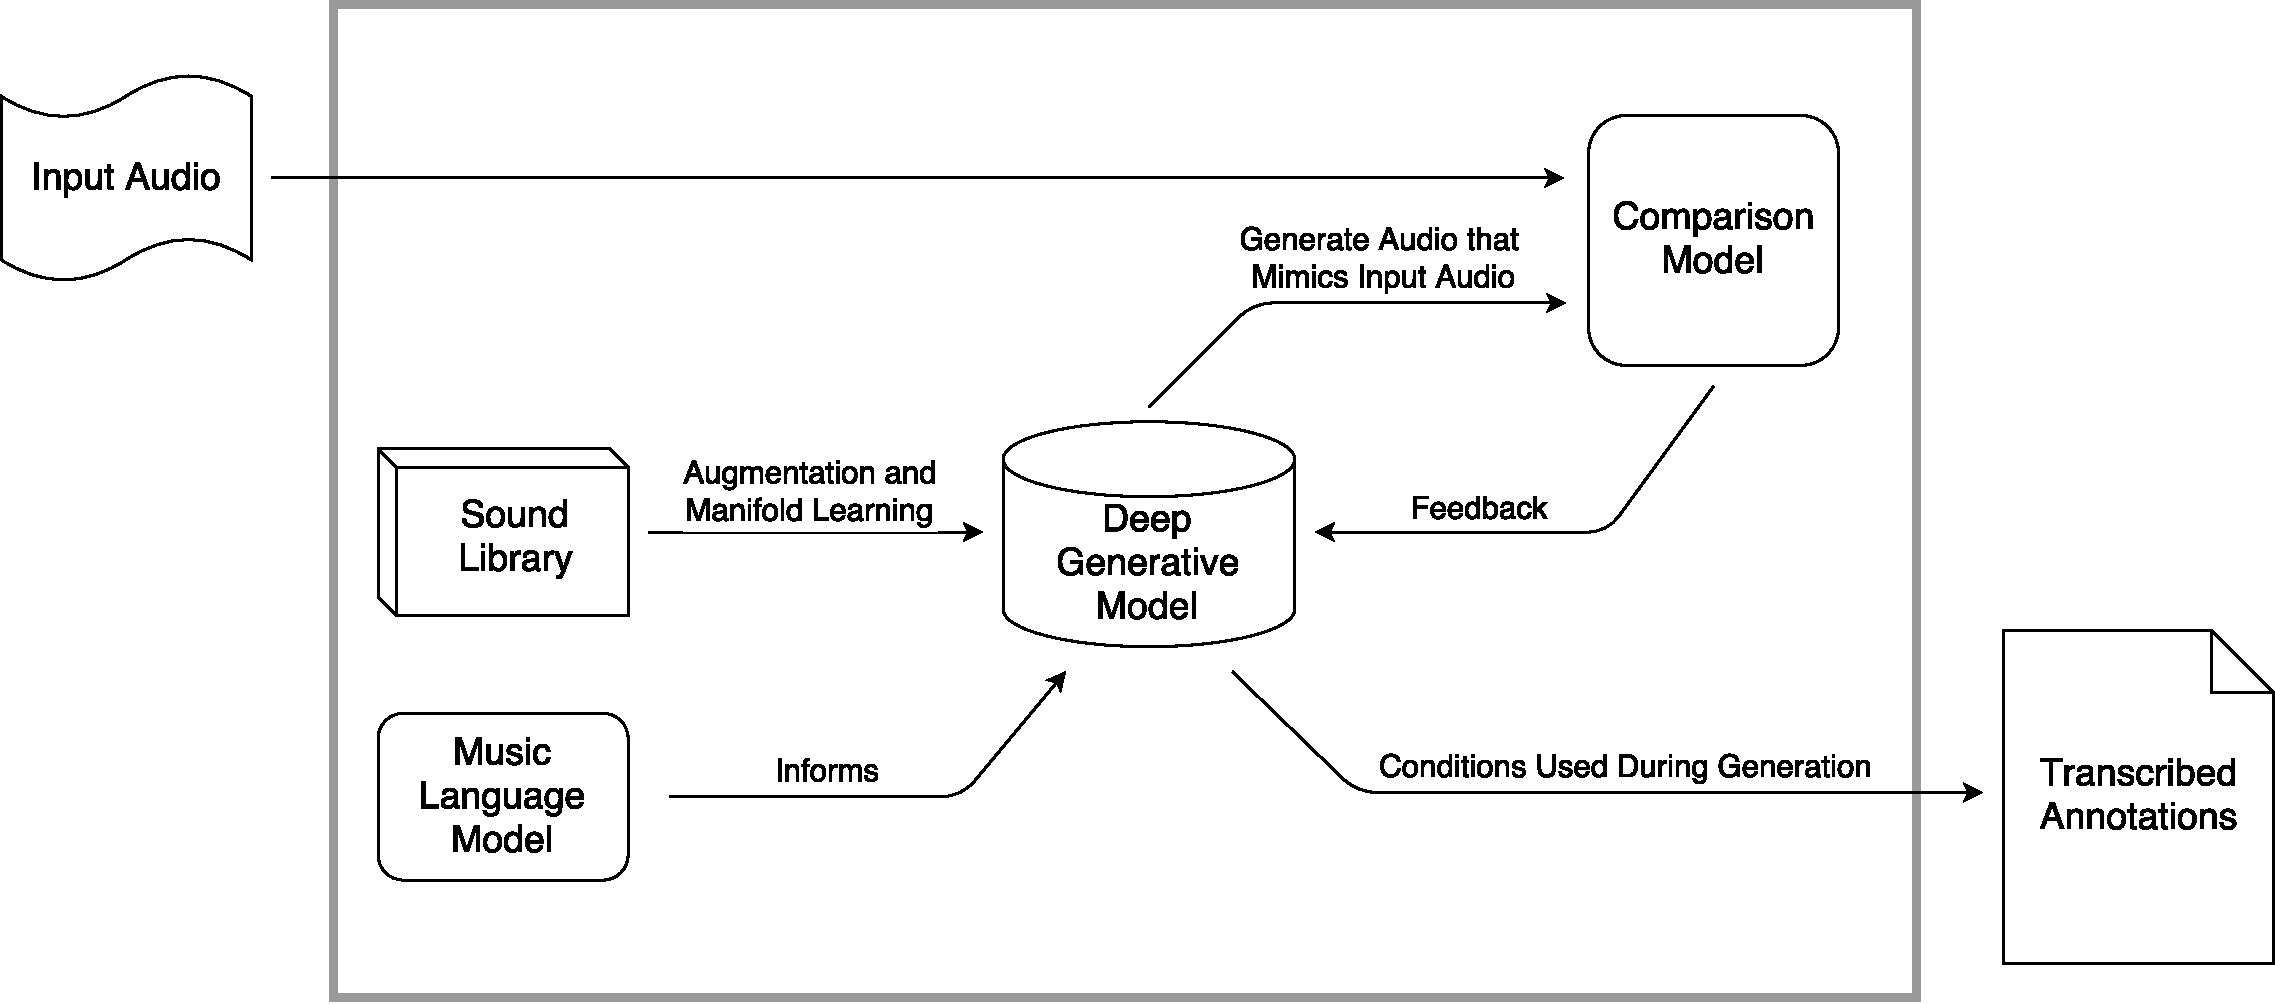
\includegraphics[width=\textwidth]{grand.pdf}
	\caption{A high-level schematic of the proposed automatic music transcription system. A deep generative model is trained using music database and music language models, to generate audio track that sounds similarly as the input audio. The conditions used to generate the matching audio can produce the predicted music transcription. }\label{fig:grand}
\end{figure}

Figure \ref{fig:grand} shows the high-level diagram for an end-to-end automatic music transcription system built around a deep generative model.
In short, the deep generative model in the center will learn to generate audio signals that mimics the input, and the combinations of instruments and pitches used for generating the audio will be the resulting transcription.
In order for the generative model to learn the semantic latent variables in music, the model needs to be able to disentangle the pitch and timbre information from the audio.
While the techniques such as batch normalization and using diagonal covariance matrices in variational autoencoders are intended to induce statistical independence between latent components,
making the components have a fully disentangled semantic information remains an active area of research.
The next section discusses the possible methods for disentanglement in the context of deep generative models.

%The proposed transcription system is not only powered by deep generative models and music language models, but also by a few other important techniques that will make the implementation possible to be realized.
%Data augmentation is a method for increasing the quantity of available data using transformations that does not alter or deterministically alter the label, and has been successfully applied to image classification tasks  \cite{krizhevsky2012imagenet}. MUDA \cite{mcfee2015muda} provides a software framework for augmenting musical audio, which supports pitch shift, time stretch, background noise, and dynamic range compression.
%It would be also possible augment to the data by filtering with the impulse responses according to various room acoustics, adding reverberations to the audio.
%Combined with the audio sources from various software instruments and sample libraries, these methods for audio augmentation can greatly increase the effective size of training data, and will help the deep model to more accurately learn the distribution of the real-world musical sounds.
%It is more efficient in terms of both time and space complexity to perform data augmentation on-the-fly instead of storing precomputed data, because the size of data increases combinatorially depending on the available augmentation schemes.


\section{Generative Models and Learning Disentangled Representations}

This section revisits the definition of generative model, whose primary focus is to model the data distribution:
\begin{equation}\label{eqn:data-distribution}
p(\mathbf{x}).
\end{equation}
The objective of AMT is to find the label (i.e. transcription) $\mathbf{y}$ corresponding to the data $\mathbf{x}$, in which case the generative model concerns the joint distribution of the data and the annotation:
\begin{equation}\label{eqn:joint-distribution}
p(\mathbf{x}, \mathbf{y}),
\end{equation}
as opposed to discriminative models which concerns the conditional distribution:
\begin{equation}\label{eqn:data-conditional-distribution}
p(\mathbf{y} | \mathbf{x}).
\end{equation}
Some deep generative models such as cGAN \cite{mirza2014conditional} can be formulated to perform a conditional generation depending on the label, effectively sampling from:
\begin{equation}\label{eqn:label-conditional-distribution}
p(\mathbf{x} | \mathbf{y}).
\end{equation}
Some may argue that this is not a true generative modeling, because the definition does not distinguish which among $\mathbf{x}$ and $\mathbf{y}$ is the label, so Equation \ref{eqn:label-conditional-distribution} should also describe a discriminative model as Equation \ref{eqn:data-conditional-distribution} does.

In this thesis, a relaxed definition of ``generative model'' will be used to classify those models as also generative, by distinguishing data and labels as:
\begin{itemize}
	\item \textbf{data}: a higher-dimensional entity that is typically observed as-is and consists of entangled representations from which it is harder to extract useful information.
	\item \textbf{label}: a lower-dimensional entity which often requires manual annotations to obtain and consists of disentangled representations from which it is easier to extract useful information.
\end{itemize}
By using this definition, a model that only performs conditional synthesis can still be called a generative model.

As emphasized in the introduction, disentanglement is the key to effectively obtaining the desired labels for AMT.
In the overview paper on representation learning, \citeA{bengio2013representation} concluded that the most robust feature learning should ``\emph{disentangle as many factors as possible, discarding as little information about the data as is practical}''.
The main hypothesis of this thesis is that generative models fit well to this objective, since they have to know all factors required for generation and have to minimize the information loss at the same time.
% The statical models for disentanglement are similar to the techniques for source separation covered in Section \ref{ch:mir}.\ref{sec:separation}, because source separation is essentially a disentanglement problem of different sources.
Deep learning models are considered to be doing particularly well in performing disentanglement, as they can learn high-level concepts from just pixel- or sample-level data examples.
\citeA{brahma2016disentanglement} studied the features learned in different layers in a deep model and observed that deeper layers gradually unfold and flatten the data distribution, building a disentangled representation.
However, it does not necessarily mean that the factors in deeper layers always contain completely isolated information of interest.

For this reason, inducing disentanglement in deep generative models has recently become an intriguing area of research.
InfoGAN \cite{chen2016infogan} is one of the most notable models that performs disentanglement in an unsupervised manner by maximizing the mutual information between a portion of latent factors and the observation.
Information dropout \cite{achille2018information} is a generalization of the standard Dropout technique that obtains more disentangled factors.
FactorVAE \cite{kim2018factor} is a VAE model that encourages the factors in variational posterior to be independent.
Other examples include DNA-GAN \cite{xiao2017dnagan} which is inspired by the mechanism of gene expression,
and semantically decomposed GAN (SD-GAN) \cite{donahue2017gan} which learns to distinguish variations in two domains by training with pairs of data examples belonging to the same category.

While there is no silver bullet yet, these studies suggest that principled considerations for achieving disentanglement should be made during the architectural design and experiments for this thesis.


\section{Methods}

This section describes the methodology and the experimental design for achieving the goals of this thesis.
There are two main subproblems defined in Section \ref{ch:introduction}.\ref{sec:subproblems}, concerning AMT using a deep generative model and using the generative component for data augmentation.
The experiments for each subproblem are designed to follow the corresponding lower-level questions, which is aimed at incrementally getting closer to the final goals.

\subsection{End-to-End Generative Model between Audio and Piano Rolls}

This task is the primary objective of this thesis, by building a bidirectional connection between the domain of audio signals and the domain of piano roll representations.
The three subtasks are designed to gradually expand the two domains, from a fixed-length monophonic notes to multi-instrument polyphonic music.

\mbox{}\\\noindent\emph{Disentangling Pitch and Timbre}\mbox{}

For the first subtask, fixed-length monophonic signals are assumed.
As \citeA{engel2017nsynth} studied the entanglement of pitch and timbre using the WaveNet architecture, the goal of this subtask is to build a deep generative model that can separately control pitch and timbre.
A preliminary architecture implementing this idea is shown in Figure \ref{fig:pegan}.
Domain-adversarial training \cite{ganin2015domain} and semantically decomposed GAN \cite{donahue2017gan} could be helpful in stable training of the proposed setup.
A shortcoming of this architecture is that each pitch values are considered as separate categories, and it could be overcome by an improved methods for conditional synthesis, such as the projection discriminator \cite{miyato2018cgan}.

\begin{figure}
	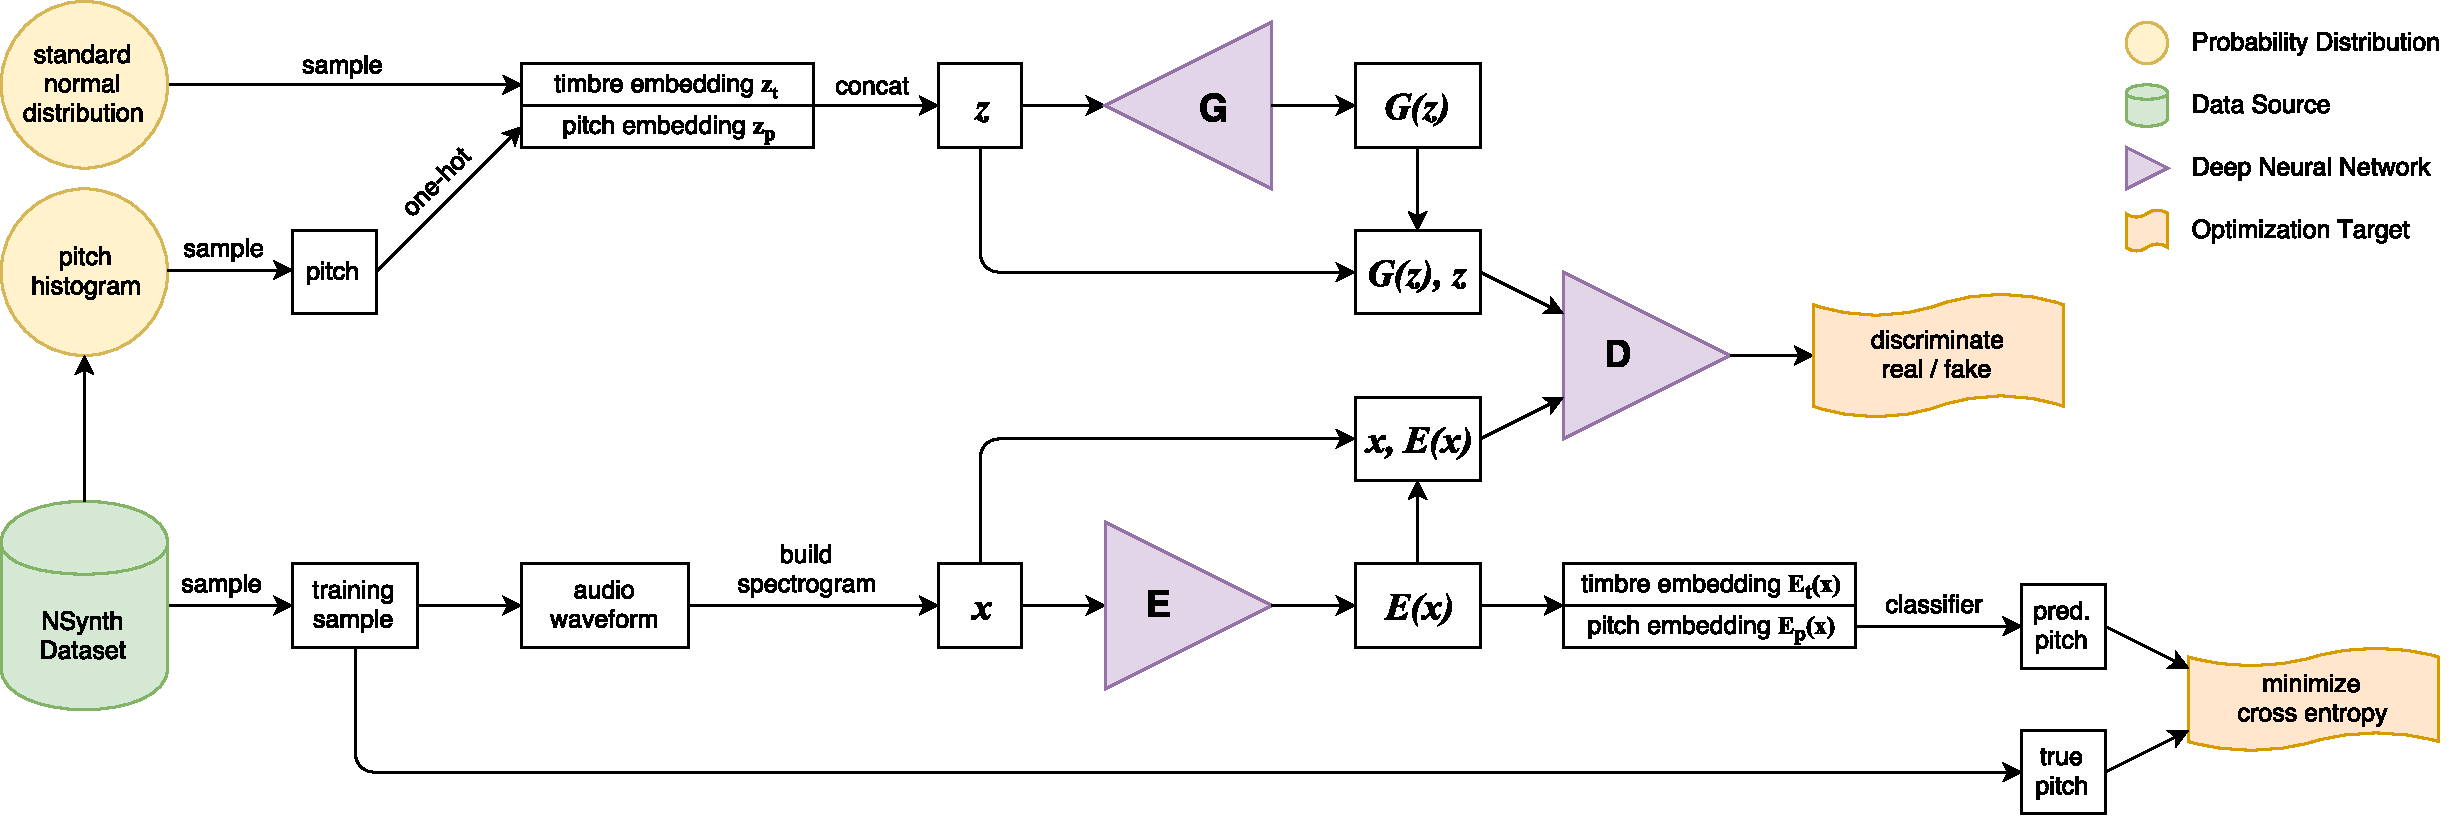
\includegraphics[width=\textwidth]{PEGAN.pdf}
	\caption{An architecture combining a conditional GAN \protect\cite{mirza2014conditional} and a bidirection GAN \protect\cite{donahue2016bigan}, which uses a concatenation of pitch and timbre embeddings to be able to control pitch and timbre separately in the generator.}
	\label{fig:pegan}
\end{figure}

\mbox{}\\\noindent\emph{Extending to Polyphony and Variable-Length Audio}\mbox{}

The next goal is to extend the generative model to deal with polyphony and variable-length audio.
In order to generalize to an arbitrary length in time, the latent representation needs to include the time dimension in addition to the pitch and timbre factors.
This is in a similar manner where \citeA{engel2017nsynth} used a generative model trained on 4-second clips to synthesize audio of a longer length.
The fully convolutional architecture \cite{shelhamer2017fcn} may be appropriate for dealing with variable-length inputs and outputs.

In order for the model to learn to separate different timbres and pitches, the transcription model may contain an addition operation which mixes multiple sources corresponding to each instrument and each note.
Such setup may not have a straightforward training scheme, in which case incorporating a clustering techniques such as expectation-maximization can be helpful.
It may be also necessary to limit the number of polyphony or instruments to have a computationally feasible solution.

\mbox{}\\\noindent\emph{Obtaining Piano Rolls from the Embeddings}\mbox{}

This task is on the ultimate problem of obtaining the per-instrument piano roll representations.
In order to achieve this, a model connecting the event-level representation to the latent embedding space is required.

\subsection{Generative Model as Augmentation}

This subproblem concerns the second objective of this thesis: using the generative component of the AMT model for data augmentation.
These tasks are auxiliary to the main objective and are also less technically challenging, while they are designed to work in conjunction with the AMT model.

\mbox{}\\\noindent\emph{Software Instrument and Audio Post-Processing}\mbox{}

This task is to reconfirm the effectiveness of data augmentation, by feeding additional training dataset consisting of sounds generated using software instruments and audio post-processing techniques.
The audio degradation toolbox \cite{mauch2013adt} and MUDA \cite{mcfee2015muda} can be utilized for simple data augmentation, and software instruments, usually packaged with specialized APIs, such as VST3 or Audio Units \cite{pirkle2014synthesizer}, can be programmed to generate various ranges of sounds to be augmented.

\mbox{}\\\noindent\emph{Incorporating a Music Language Model}\mbox{}

This subtask concerns the application of a music language model that serves as a sensible prior to the output of the generative AMT model.
Designing a music language model itself is an intriguing problem, but for the purpose of this thesis, existing music sequence generation models such as MidiNet \cite{yang2017midinet} or MuseGan \cite{dong2017musegan} can be incorporated.

\mbox{}\\\noindent\emph{Positive Feedback Cycle between Transcription and Augmentation}\mbox{}

This last task would be an integration of all of the above methods, to build an architecture where the improved generative model serves as a better augmentation tool, which helps the AMT model achieve improved transcription performance.


\subsection{Expected Challenges}

Regretfully, the above descriptions of the experimental designs do not fully specify the model architecture and representation, because the biggest challenges lie on finding the exact architecture and representation that works.
One such challenge is the size of the representation; generative adversarial networks are the only deep generative models that have meaningfully generated images larger than 128$\times$128 pixels, however the training dynamics of GANs become increasingly unstable as the size of the representation gets larger.
In order to train a GAN that deals with a sufficient size of audio representation, it may be necessary to employ more intricate architectures such as progressive growing \cite{karras2017pggan}.
Another obstacle is the flood of GAN models, making it difficult to determine the correct architecture to work with.
Deeper theoretical understanding and empirical knowledge on GAN training would be required.

\section{Evaluation}

The performance of multiple fundamental frequency estimation in the form of piano rolls are evaluated in a number of different ways.
The simplest metric is the frame-level accuracy, which measures the portion of the correct predictions 
\begin{equation}
\mathrm{Accuracy} = \frac{\sum_{t=1}^T TP(t)}{\sum_{t=1}^T \left ( TP(t) + FP(T) + FN(t) \right ) },
\end{equation}
where TP, FP, and FN refers to true positives, false positives, and false negatives, respectively.

Additional evaluation metrics have been proposed in \cite{poliner2007piano} to reflect three different types of transcription errors, a missed error where the system fails to predict a pitch at all, a substitution error where a different F0 is predicted, and a false alarm where the system predicts a pitch that is not actually present:
\begin{eqnarray}
E_{tot} & = & \frac{\sum_{t=1}^T \max ( N_{ref}(t), N_{sys}(t) ) - N_{corr}(t)}{\sum_{t=1}^T N_{ref}(t)}, \\
E_{sub} & = & \frac{\sum_{t=1}^T \min ( N_{ref}(t), N_{sys}(t) ) - N_{corr}(t)}{\sum_{t=1}^T N_{ref}(t)}, \\
E_{miss} & = & \frac{\sum_{t=1}^T \max ( 0, N_{ref}(T) - N_{sys}(t) )}{\sum_{t=1}^T N_{ref}(t)}, \\
E_{fa} & = &  \frac{\sum_{t=1}^T \max ( 0, N_{sys}(T) - N_{ref}(t) )}{\sum_{t=1}^T N_{ref}(t)},
\end{eqnarray}
where $N_{ref}(t)$ the number of ground-truth f0s at frame $t$, $N_{sys}$ is the number of reported f0s, and $N_{corr}(t)$ is the number of correctly predicted f0s.
These errors are useful, because they enable a comparison of multi-pitch estimation systems with respect to the different types of errors \cite{bay2009evaluation}.
The open-source implementation in the \texttt{mir\_eval} package \cite{raffel2014mir_eval} will be used for convenience and reproducibility.

\section{Datasets}

Based on the assumptions on the scope of music discussed in Section \ref{ch:introduction}.\ref{sec:limitations}, datasets that contain non-vocal harmonic instrumental sounds without excessive variations in timbre are desirable.
For early experiments, the NSynth Dataset published recently by Google's Magenta project \cite{engel2017nsynth} is appropriate, as the dataset contains additional kinds of instruments and comes with more accurate annotations.
As discussed above, open-source and commercial software instruments and effects can also be used.

In order to compare the performance of the proposed AMT model with existing transcription methods, the standard benchmark datasets containing polyphonic classical instruments such as MAPS \cite{emiya2010multipitch}, Bach10 \cite{duan2010bach10}, and MusicNet \cite{thickstun2017musicnet} are good choices.

%!TEX root = ../dissertation.tex

\graphicspath{{5-pilot/figures/}}
\newcommand\firstpilottitle{ Convolutional Representation for Pitch Estimation }
\chapter[Pilot Study 1: \newline \firstpilottitle]{~~~~~~~~~~~~~~~~~~~~~~~~~~~~~~~~~Pilot Study 1: \newline\vspace{-0.5em}\newline \firstpilottitle}
\label{ch:pilot}


In this chapter, a preliminary research result toward the direction of the thesis is presented, focusing on a pitch tracking algorithm based on one-dimensional convolutional neural networks.
While not directly being a part of the overall system as described in Figure \ref{fig:grand}, these experiments are expected to provide valuable insights about what convolutional representations can learn from music audio signals, and how their architecture should be designed to maximize the effectiveness.
The work in the following sections are featured in \cite{kim2018crepe}.


\section{Introduction}\label{sec:introduction}

Estimating the fundamental frequency (f0) of a monophonic audio signal, also known as pitch tracking or pitch estimation, is a long-standing topic of research in audio signal processing.
Pitch estimation plays an important role in music signal processing, where monophonic pitch tracking is used as a method to generate pitch annotations for multi-track datasets \cite{bittner2014medleydb} or as a core component of melody extraction systems \cite{bosch2014melody, mauch2015computer}. 
Pitch estimation is also important for speech analysis, where prosodic aspects such as intonations may reflect various features of speech \cite{zubizarreta1998prosody}.

Pitch is defined as a subjective quality of perceived sounds and does not precisely correspond to the physical property of the fundamental frequency \cite{hartmann1997signals}.
However, apart from a few rare exceptions, pitch can be quantified using fundamental frequency, and thus they are often used interchangeably outside psychoacoustical studies. 
For convenience, the two terms are interchangeably throughout this chapter.

Computational methods for monotonic pitch estimation have been studied for more than a half-century \cite{noll1967cepstrum}, and many reliable methods have been proposed since.
Earlier methods commonly employ a certain candidate-generating function, accompanied by pre- and post-processing stages to produce the pitch curve.
Those functions include the cepstrum \cite{noll1967cepstrum}, the autocorrelation function (ACF) \cite{dubnowski1976acf}, the average magnitude difference function (AMDF) \cite{ross1974amdf}, the normalized cross-correlation function (NCCF) as proposed by RAPT \cite{talkin1995rapt} and PRAAT \cite{boersma1993praat}, and the cumulative mean normalized difference function as proposed by YIN \cite{decheveigne2002yin}. More recent approaches include SWIPE \cite{camacho2008swipe}, which performs template matching with the spectrum of a sawtooth waveform, and 
pYIN \cite{mauch2014pyin}, a probabilistic variant of YIN that uses a Hidden Markov Model (HMM) to decode the most probable sequence of pitch values.
According to a few comparative studies, the state of the art is achieved by YIN-based methods \cite{von2010comparison, babacan2013comparative}, with pYIN being the best performing method to date \cite{mauch2014pyin}.

A notable trend in the above methods is that the derivation of a better pitch detection system solely depends on cleverly devising a robust candidate-generating function and/or sophisticated post-processing steps, i.e.~heuristics, and none of them are directly learned from data, except for manual hyperparameter tuning.
This contrasts with many other problems in music information retrieval like chord ID \cite{humphrey2012rethinking} and beat detection \cite{bock2011enhanced}, where data-driven methods have been shown to consistently outperform heuristic approaches.
One possible explanation for this is that since fundamental frequency is a low-level physical attribute of an audio signal which is directly related to its periodicity, in many cases heuristics for estimating this periodicity perform extremely well with accuracies (measured in raw pitch accuracy, defined later on) close to 100\%, leading some to consider the task a solved problem.
This, however, is not always the case, and even top performing algorithms like pYIN can still produce noisy results for challenging audio recordings such as a sound of uncommon instruments or a pitch curve that fluctuates very fast.
This is particularly problematic for tasks that require a flawless f0 estimation, such as using the output of a pitch tracker to generate reference annotations for melody and multi-f0 estimation \cite{salamon2017analysis,bittner2017deepsalience}.

In this chapter, a novel, data-driven method for monophonic pitch tracking based on a deep convolutional neural network operating on the time-domain signal is presented.
This approach, CREPE (Convolutional  Representation  for  Pitch  Estimation), obtains state-of-the-art results, outperforming heuristic approaches such as pYIN and SWIPE while being more robust to noise too.
It is further shown that CREPE is highly precise, maintaining over 90\% raw pitch accuracy even for a strict evaluation threshold of just 10 cents.
The Python implementation of the proposed approach, along with a pre-trained model of CREPE are made available online\footnote{\texttt{https://github.com/marl/crepe}} for easy utilization and reproducibility.

\section{Architecture}

\begin{figure*}
	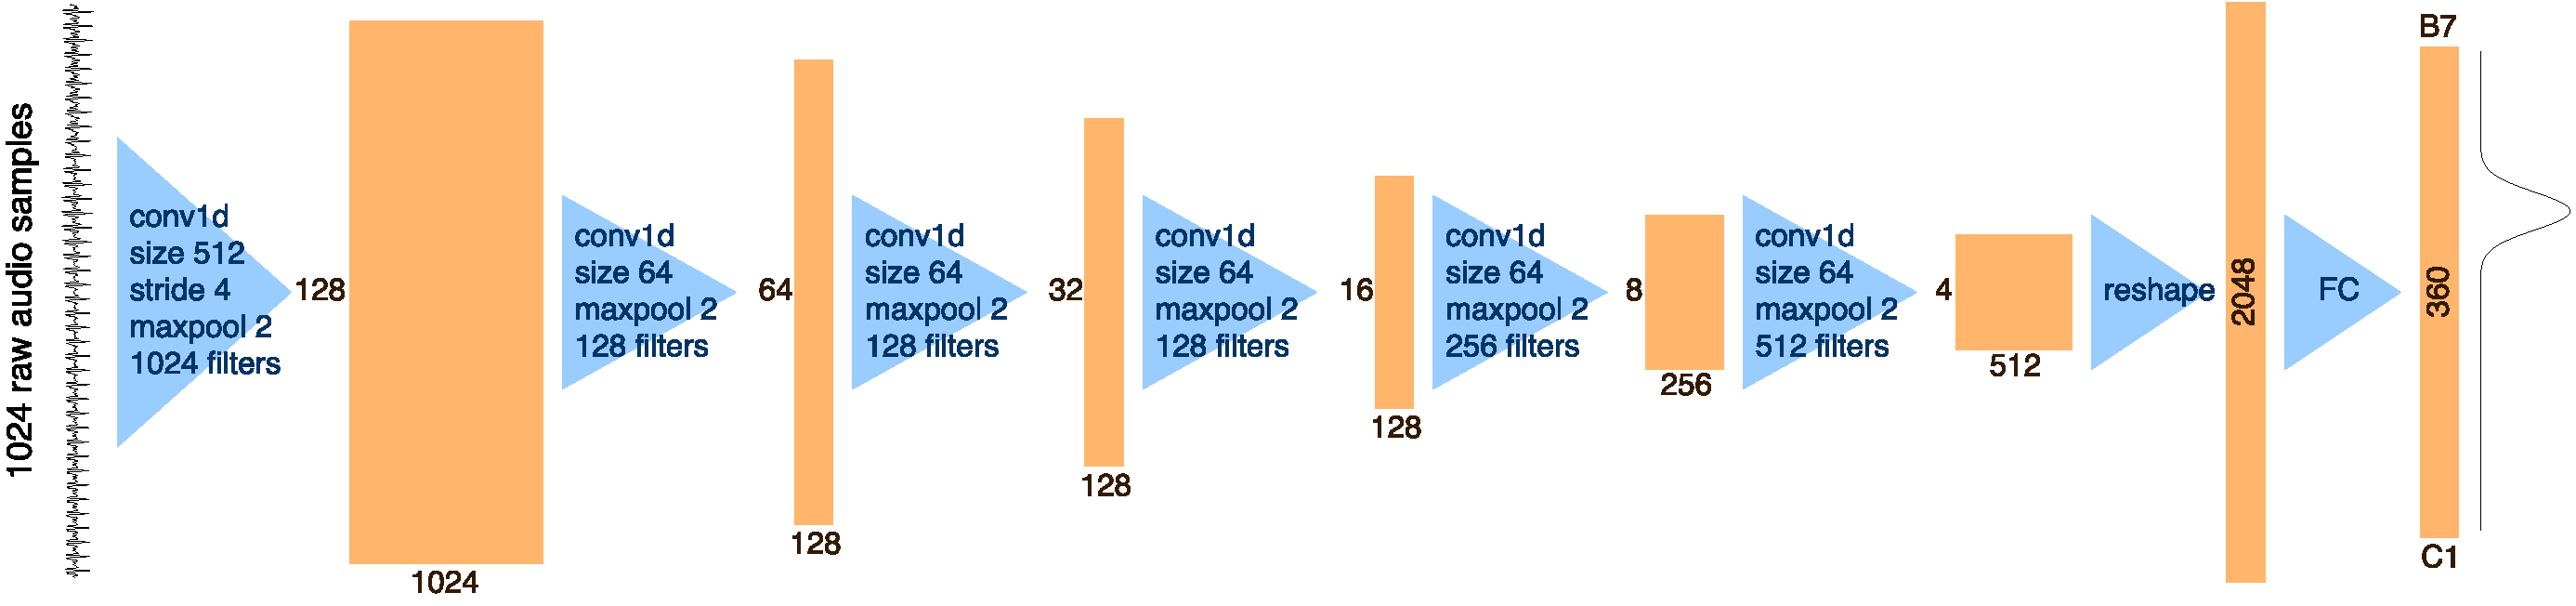
\includegraphics[width=\textwidth]{architecture.pdf}
	\caption{The architecture of the CREPE pitch tracker. The six convolutional layers operate directly on the time-domain audio signal, producing an output vector that approximates a Gaussian curve as in Equation \ref{eqn:gaussian}, which is then used to derive the exact pitch estimate as in Equation \ref{eqn:resulting}.}
	\label{fig:architecture}
\end{figure*}

CREPE consists of a deep convolutional neural network which operates directly on the time-domain audio signal to produce a pitch estimate.
A block diagram of the proposed architecture is provided in Figure \ref{fig:architecture}.
The input is a 1024-sample excerpt from the time-domain audio signal, using a 16 kHz sampling rate.
There are six convolutional layers that result in a 2048-dimensional latent representation, which is then connected densely to the output layer with sigmoid activations corresponding to a 360-dimensional output vector $\hat{\mathbf{y}}$.
From this, the resulting pitch estimate is calculated deterministically.

Each of the 360 nodes in the output layer corresponds to a specific pitch value, defined in cents.
Cent is a unit representing musical intervals relative to a reference pitch $f_{\mathrm{ref}}$ in Hz, defined as a function of frequency $f$ in Hz:
\begin{equation}
\cent(f) = 1200 \cdot \log_2 \frac{f}{f_{\mathrm{ref}}},
\end{equation}
where $f_{\mathrm{ref}} = 10 \mathrm{~Hz}$ throughout the experiments. 
This unit provides a logarithmic pitch scale where 100 cents equal one semitone.
The 360 pitch values are denoted as $\cent_1, \cent_2, \cdots, \cent_{360}$ and are selected so that they cover six octaves with 20-cent intervals between C1 and B7, corresponding to 32.70 Hz and 1975.5 Hz. 
The resulting pitch estimate $\hat{\cent}$ is the weighted average of the associated pitches $\cent_i$ according to the output $\hat{\mathbf{y}}$, which gives the frequency estimate in Hz:
\begin{equation}\label{eqn:resulting}
\hat{\cent} = \frac{\sum_{i=1}^{360}\hat{y}_i \cent_i}{\sum_{i=1}^{360} \hat{y}_i}, ~~~~~~~~~~~~~~
\hat{f} = f_{\mathrm{ref}} \cdot 2 ^ {\hat{\cent} / 1200}.
\end{equation}

The target outputs we use to train the model are 360-dimensional vectors, where each dimension represents a frequency bin covering 20 cents (the same as the model's output).
The bin corresponding to the ground truth fundamental frequency is given a magnitude of one.
As in \cite{bittner2017deepsalience}, in order to soften the penalty for near-correct predictions, the target is Gaussian-blurred in frequency such that the energy surrounding a ground truth frequency decays with a standard deviation of 25 cents:
\begin{equation}\label{eqn:gaussian}
y_i = \exp \left ( {-\frac{(\cent_i - \cent_{\mathrm{true}})^2}{2 \cdot 25^2}} \right ),
\end{equation}
This way, high activations in the last layer indicate that the input signal is likely to have a pitch that is close to the associated pitches of the nodes with high activations.

The network is trained to minimize the binary cross entropy between the target vector $\mathbf{y}$ and the predicted vector $\mathbf{\hat{y}}$:
\begin{equation}
\mathcal{L}(\mathbf{y}, \mathbf{\hat{y}}) = \sum_{i=1}^{360} \left ( - y_i \log \hat{y_i} - (1 - y_i) \log (1 - \hat{y_i}) \right ),
\end{equation}
where both $y_i$ and $\hat{y}_i$ are real numbers between 0 and 1.
This loss function is optimized using the ADAM optimizer \cite{kingma2015adam}, with the learning rate 0.0002. 
The best performing model is selected after training until the validation accuracy no longer improves for 32 epochs, where one epoch consists of 500 batches of 32 examples randomly selected from the training set. 
Each convolutional layer is preceded with batch normalization \cite{ioffe2015batchnorm} and followed by a dropout layer \cite{srivastava2014dropout} with the dropout probability 0.25.
This architecture and the training procedures are implemented using Keras \cite{chollet2015keras}.




\section{Experiments}

\subsection{Datasets}

In order to objectively evaluate CREPE and compare its performance to alternative algorithms, we require audio data with perfect ground truth annotations.
This is especially important since the performance of the compared algorithms is already very high.
In light of this, we cannot use a dataset such as MedleyDB \cite{bittner2014medleydb}, since its annotation process includes manual corrections which do not guarantee a 100\% perfect match between the annotation and the audio, and it can be affected, to a degree, by human subjectivity.
To guarantee a perfectly objective evaluation, we must use datasets of synthesized audio in which we have perfect control over the f0 of the resulting signal.
We use two such datasets: the first, RWC-synth, contains 6.16 hours of audio synthesized from the RWC Music Database \cite{goto2002rwc} and is used to evaluate pYIN in \cite{mauch2014pyin}.
It is important to note that the signals in this dataset were synthesized using a fixed sum of a small number of sinusoids, meaning that the dataset is highly homogenous in timbre and represents an over-simplified scenario.
To evaluate the algorithms under more realistic (but still controlled) conditions, the second dataset we use is a collection of 230 monophonic stems taken from MedleyDB and re-synthesized using the methodology presented in \cite{salamon2017analysis}, which uses an analysis/synthesis approach to generate a synthesized track with a perfect f0 annotation that maintains the timbre and dynamics of the original track.
This dataset consists of 230 tracks with 25 instruments, totaling 15.56 hours of audio, and henceforth referred to as MDB-stem-synth.


\begin{figure*}[b!]
	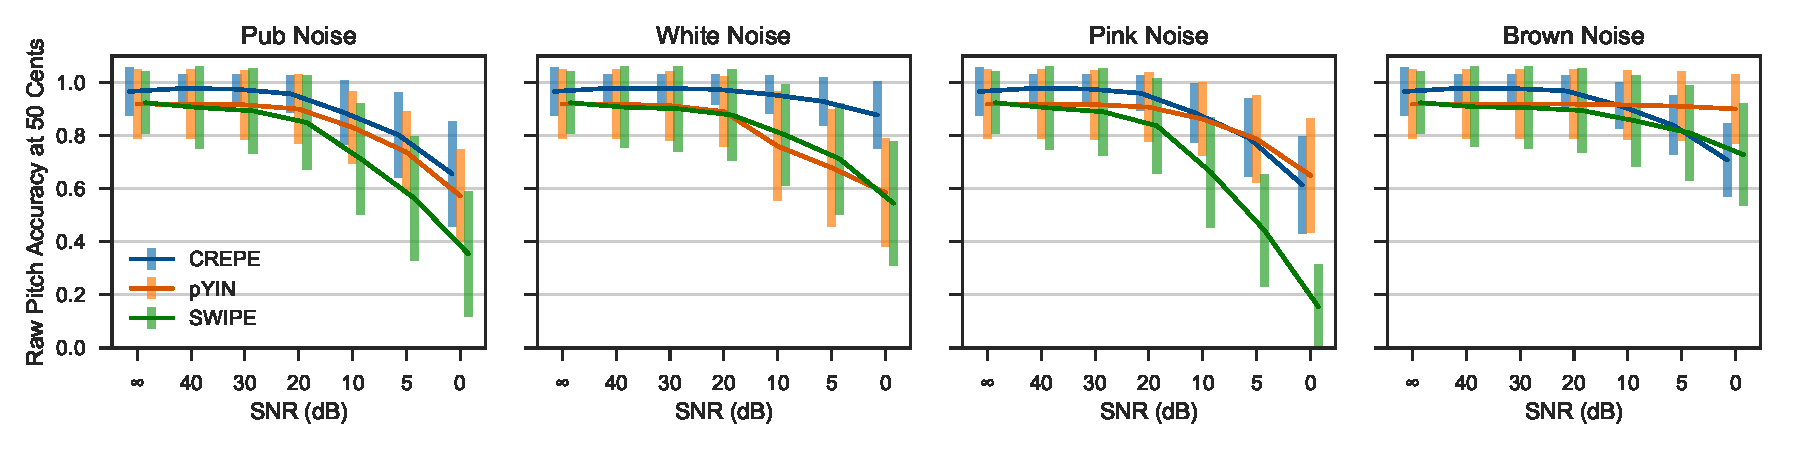
\includegraphics[width=\textwidth]{noise.pdf}
	\caption{Pitch tracking performance when additive noise signals are present. The error bars are centered at the average raw pitch accuracies and span the first standard deviations. With brown noise being a notable exception, CREPE shows the highest noise robustness in general. }
	\label{fig:noise}
\end{figure*}


\subsection{Methodology}

We train the model using 5-fold cross-validation, using a 60/20/20 train, validation, and test split.
For MDB-stem-synth, we use artist-conditional folds, in order to avoid training and testing on the same artist which can result in artificially high performance due to artist or album effects \cite{sturm2013classification}.
The evaluation of an algorithm's pitch estimation is measured in raw pitch accuracy (RPA) and raw chroma accuracy (RCA) with 50 cent thresholds \cite{salamon2014melody}.
These metrics measure the proportion of frames in the output for which the output of the algorithm is within 50 cents (a quarter-tone) of the ground truth.
We use the reference implementation provided in \texttt{mir\_eval} \cite{raffel2014mir_eval} to compute the evaluation metrics.

We compare CREPE against the current state of the art in monophonic pitch tracking, represented by the pYIN \cite{mauch2014pyin} and SWIPE \cite{camacho2008swipe} algorithms.
To examine the noise robustness of each algorithm, we also evaluate their pitch tracking performance on degraded versions of MDB-stem-synth, using the Audio Degradation Toolbox (ADT) \cite{mauch2013adt}.
We use four different noise sources provided by the ADT: pub, white, pink, and brown.
The pub noise is an actual recording of the sound in a crowded pub, 
and the white noise is a random signal with a constant power spectral density over all frequencies.
The pink and brown noise have the highest power spectral density in low frequencies, and the densities fall off at 10 dB and 20 dB per decade respectively.
Seven different signal-to-noise ratio (SNR) values are used: $\infty$, 40, 30, 20, 10, 5, and 0 dB.


\subsection{Results}

\subsubsection{Pitch Accuracy}

Table \ref{tbl:accuracy50} shows the pitch estimation performance tested on the two datasets.
On the RWC-synth dataset, CREPE yields a close-to-perfect performance where the error rate is lower than the baselines by more than an order of magnitude.
While these high accuracy numbers are encouraging, those are achievable thanks to the highly homogeneous timbre of the dataset.
In order to test the generalizability of the algorithms on a more timbrally diverse dataset, the performance is evaluated on the MDB-stem-synth dataset as well.
It is notable that the degradation of performance from RWC-synth is more significant for the baseline algorithms, implying that CREPE is more robust to complex timbres compared to pYIN and SWIPE.

Finally, to see how the algorithms compare under scenarios where any deviation in the estimated pitch from the true value could be detrimental, Table \ref{tbl:thresholds} reports the RPA at lower evaluation tolerance thresholds of 10 and 25 cents as well as the RPA at the standard 50 cents threshold for reference.
The table indicates that as the threshold is decreased, the difference in performance becomes more accentuated, with CREPE 
%maintaining near-perfect RPA for RWC-synth while the others degrade significantly.
outperforming by over 8 percentage points when the evaluation tolerance is lowered to 10 cents.
This suggests that CREPE is especially preferable when even minor deviations from the true pitch should be avoided as best as possible.
Obtaining highly precise pitch annotations is perceptually meaningful for transcription and analysis/resynthesis applications.


\subsubsection{Noise Robustness}

Noise robustness is key to many applications like speech analysis for mobile phones or smart speakers, or for live music performance.
Figure \ref{fig:noise} shows how the pitch estimation performance is affected when an additive noise is present in the input signal.
CREPE maintains the highest accuracy for all SNR levels for pub noise and white noise, and for all SNR levels except for the highest level of pink noise.
Brown noise is the exception where pYIN's performance is almost unaffected by the noise.
This can be attributed to the fact that brown noise has most of its energy at low frequencies, to which the YIN algorithm (on which pYIN is based) is particularly robust.

To summarize, CREPE performs better in all cases where the SNR is below 10 dB while the performance varies depending on the spectral properties of the noise when the noise level is higher, which indicates that this approach can be reliable under a reasonable amount of additive noise.
CREPE is also more stable, exhibiting consistently lower variance in performance compared to the baseline algorithms.


\begin{table}[t]
	\begin{center}
		\begin{tabular}{c|c||c|c|c} \hline
			\multicolumn{1}{c}{Dataset} & \multicolumn{1}{c}{Metric} & \multicolumn{1}{c}{CREPE} & \multicolumn{1}{c}{pYIN} & \multicolumn{1}{c}{SWIPE} \\ \hline
			\multirow{2}{*}{RWC-synth} & RPA & \textbf{0.999$\pm$0.002} & 0.990$\pm$0.006& 0.963$\pm$0.023 \\ \cline{2-5}
			& RCA & \textbf{0.999$\pm$0.002} & 0.990$\pm$0.006& 0.966$\pm$0.020 \\ \hline \hline
			\multirow{2}{*}{MDB-stem-synth} & RPA & \textbf{0.967$\pm$0.091} & 0.919$\pm$0.129& 0.925$\pm$0.116 \\ \cline{2-5}
			& RCA & \textbf{0.970$\pm$0.084} & 0.936$\pm$0.092& 0.936$\pm$0.100 \\ \hline
		\end{tabular}
	\end{center}
	\caption{Average raw pitch/chroma accuracies and their standard deviations, tested with the 50 cents threshold.}
	\label{tbl:accuracy50}
\end{table}

\begin{table}[t]
	\begin{center}
		\begin{tabular}{c|c||c|c|c} \hline
			\multicolumn{1}{c}{Dataset} & \multicolumn{1}{c}{Threshold} &  \multicolumn{1}{c}{CREPE} & \multicolumn{1}{c}{pYIN} & \multicolumn{1}{c}{SWIPE} \\ \hline
			
			\multirow{3}{*}{RWC-synth} 
			& 50 cents & \textbf{0.999$\pm$0.002} & 0.990$\pm$0.006 & 0.963$\pm$0.023 \\ \cline{2-5}
			& 25 cents & \textbf{0.999$\pm$0.003} & 0.972$\pm$0.012 & 0.949$\pm$0.026 \\ \cline{2-5}
			& 10 cents & \textbf{0.995$\pm$0.004} & 0.908$\pm$0.032 & 0.833$\pm$0.055 \\ \hline \hline
			
			\multirow{3}{*}{MDB-stem-synth}
			& 50 cents & \textbf{0.967$\pm$0.091} & 0.919$\pm$0.129 & 0.925$\pm$0.116 \\ \cline{2-5}
			& 25 cents & \textbf{0.953$\pm$0.103} & 0.890$\pm$0.134 & 0.897$\pm$0.127 \\ \cline{2-5}
			& 10 cents & \textbf{0.909$\pm$0.126} & 0.826$\pm$0.150 & 0.816$\pm$0.165 \\ \hline
		\end{tabular}
	\end{center}
	\caption{Average raw pitch accuracies and their standard deviations, with different evaluation thresholds.}
	\label{tbl:thresholds}
\end{table}

\begin{figure*}[t]
	\begin{minipage}{\columnwidth}
		\begin{center}
			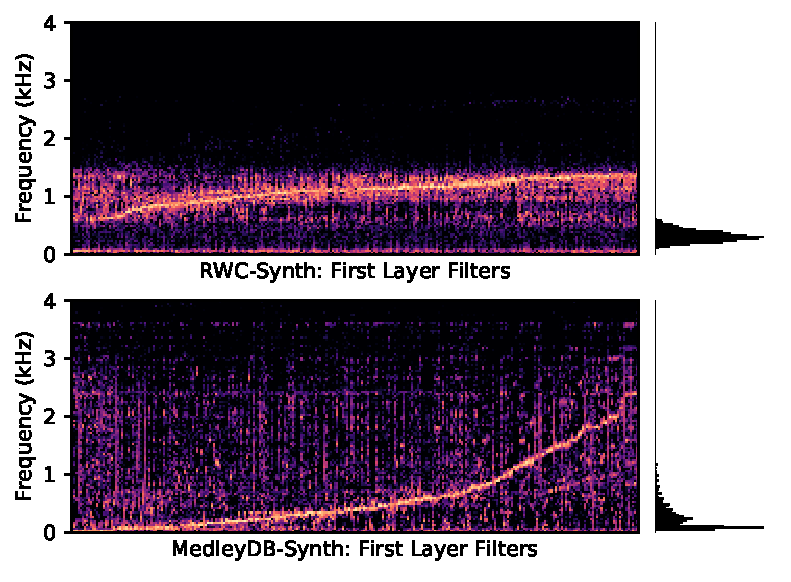
\includegraphics[width=0.8\columnwidth]{firstlayer-45.pdf}
		\end{center}
		\vspace{-10pt}
		\caption{
			Fourier spectra of the first-layer filters sorted by the frequency of the peak magnitude.
			Histograms on the right show the distribution of ground-truth frequencies in the corresponding dataset.
		}
		\label{fig:firstlayer}
	\end{minipage}
	\\ \vspace{2em} \\ 
	\begin{minipage}{\columnwidth}
		\begin{center}
			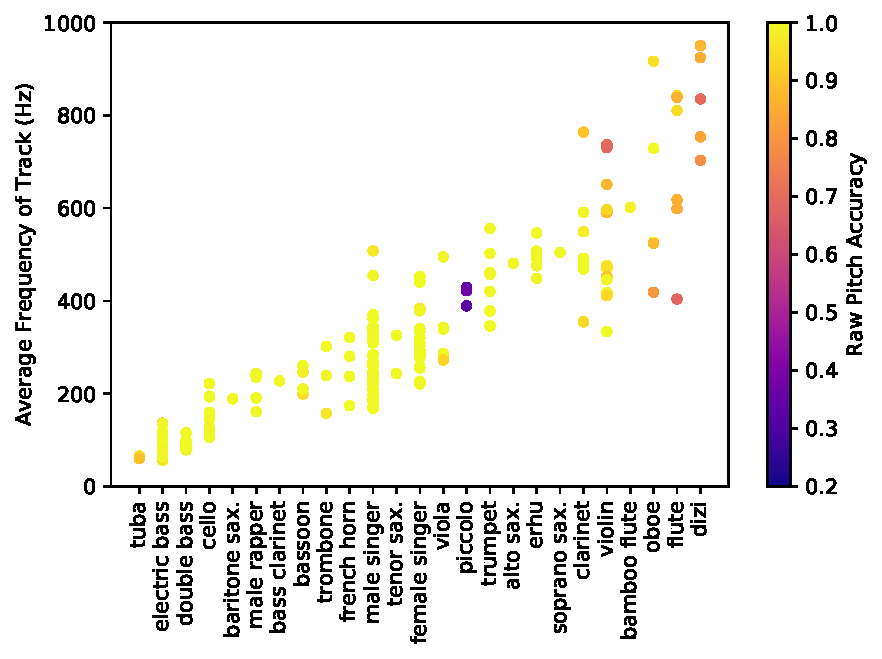
\includegraphics[width=0.8\columnwidth]{per-track-inst-45.pdf}
		\end{center}
		\vspace{-10pt}
		\caption{
			The raw pitch accuracy (RPA) of CREPE's predictions on each of the 230 tracks in MDB-stem-synth with respect to the instrument, sorted by the average frequency.
			% The  low-performing  cases  are  concentrated  in  the extreme frequencies, showing that the model performs better for the sfrequency range that are well-represented in the training set.
		}
		\label{fig:per-track}
	\end{minipage}
\end{figure*}


\subsubsection{Model Analysis}

To gain some insight into the CREPE model, Figure \ref{fig:firstlayer} visualizes the spectra of the 1024 convolutional filters in the first layer of the neural network, with histograms of the ground-truth frequencies to the right of each plot.
It is noticeable that the filters learned from the RWC-synth dataset have the spectral density concentrated between 600 Hz and 1500 Hz, while the ground-truth frequencies are mostly between 100 Hz and 600 Hz.
This indicates that the first convolutional layer in the model learns to distinguish the frequencies of the overtones rather than the fundamental frequency.
These filters focusing on overtones are also visible for MDB-stem-synth, where peak frequencies of the filters range well above the f0 distribution of the dataset, but in this case, the majority of the filters overlap with the ground-truth distribution, unlike RWC-synth.
A possible explanation for this is that since the timbre in RWC-synth is fixed and identical for all tracks, the model is able to obtain a highly accurate estimate of the f0 by modeling its harmonics.
Conversely, when the timbre is heterogeneous and more complex, as is the case for MDB-stem-synth, the model cannot rely solely on the harmonic structure and requires filters that capture the f0 periodicity directly in addition to the harmonics.
In both cases, this suggests that the neural network can adapt to the distribution of timbre and frequency in the dataset of interest, which in turn contributes to the higher performance of CREPE compared to the baseline algorithms.

\subsubsection{Performance by Instrument}

The MDB-stem-synth dataset contains 230 tracks from 25 different instruments, where electric bass (58 tracks) and male singer (41 tracks) are the most common while there are instruments that occur in only one or two tracks.
Figure \ref{fig:per-track} plots the performance of CREPE on each of the 230 tracks, with respect to the instrument of each track.
It is notable that the model performs worse for the instruments with higher average frequencies, but the performance is also dependent on the timbre.
CREPE performs particularly worse on the tracks with the dizi, a Chinese transverse flute, because the tracks came from the same artist, and they are all placed in the same split.
This means that for the fold in which the dizi tracks are in the test set, the training and validation sets do not contain a single dizi track, and the model fails to generalize to this previously unseen timbre.
There are 5 instruments (bass clarinet, bamboo flute, and the family of saxophones) that occur only once in the dataset, but their performance is decent, because their timbres do not deviate too far from other instruments in the dataset.
For the flute and the violin, although there are many tracks with the same instrument in the training set, the performance is low when the sound in the tested tracks is too low (flute) or too high (violin) compared to other tracks of the same instruments.
The low performance on the piccolo tracks is due to an error in the dataset where the annotation is inconsistent with the correct pitch range of the instrument.
Unsurprisingly, the model performs well on test tracks whose timbre and frequency range are well-represented in the training set.

\section{Discussions and Conclusion}

This chapter presented a novel data-driven method for monophonic pitch tracking based on a deep convolutional neural network operating on time-domain input, CREPE.
CREPE obtains state-of-the-art results, outperforming pYIN and SWIPE on two datasets with homogeneous and heterogeneous timbre respectively.
Furthermore, CREPE remains highly accurate even at a very strict evaluation threshold of just 10 cents.
It is also shown that in most cases CREPE is more robust to added noise.


Ideally, it is desirable to have the model invariant to all transformations that do not affect pitch, such as changes due to distortion and reverberation.
Some invariance can be induced by the architectural design of the model, such as the translation invariance induced by pooling layers in the model as well as in deep image classification models.
However, it is not as straightforward to design the model architecture to specifically ignore other pitch-preserving transformations.
While it is still an intriguing problem to build an architecture to achieve this, one could use data augmentation to generate transformed and degraded inputs that can effectively make the model learn the invariance.
The robustness of the model could also be improved by applying pitch-shifts as data augmentation \cite{mcfee2015muda} to cover a wider pitch range for every instrument.
In addition to data augmentation, various sources of audio timbre can be obtained from software instruments; NSynth \cite{engel2017nsynth} is an example where the training dataset is generated from the sound of software instruments.


Pitch values tend to be continuous over time, but CREPE estimates the pitch of every frame independently without using any temporal tracking, unlike pYIN which exploits this by using an HMM to enforce temporal smoothness.
One may potentially improve the performance of CREPE even further by enforcing temporal smoothness.
Future work includes achieving this by means of adding recurrent architecture to the model, which could be trained jointly with the convolutional front-end in the form of a convolutional-recurrent neural network (CRNN).

%!TEX root = ../dissertation.tex

\graphicspath{{6-pilot/figures/}}

\newcommand\secondpilottitle{ Deep Generative Pitch and Timbre Modeling }
\chapter[Pilot Study 2: \newline \secondpilottitle]{~~~~~~~~~~~~~~~~~~~~~~~~~~~~~~~~~Pilot Study 2: \newline\vspace{-0.5em}\newline \secondpilottitle}
\label{ch:pilot2}

\TODO{this chapter is to be expanded}

\section{Generative Adversarial Network of Instrumental Sounds}


As seen in Chapter \ref{ch:deeplearning}, the recent surge of GAN variants have shown many promising results in computer vision.
To examine the potential applicability of a GAN model in music, a few attempts were made to train GANs that learns from musical sounds, in the form of raw audio waveforms and magnitude spectrograms.
A difference between audio and images is that audio has much more high-dimensional data than the typical images used in deep learning.
Time domain signals have tens of thousands of numbers for a second of audio, and a typical resolution of a magnitude spectrogram ranges from 512 to 1024 vertical pixels where many image datasets for deep learning is under 96 pixels.
Despite this difficulty, a careful design using mode regularized generative adversarial network (MRGAN) \cite{che2016mrgan} could achieve a stable convergence of 512-by-64 images of magnitude spectrograms, as shown in Figure \ref{fig:gan}.

\begin{figure}
	\centering
	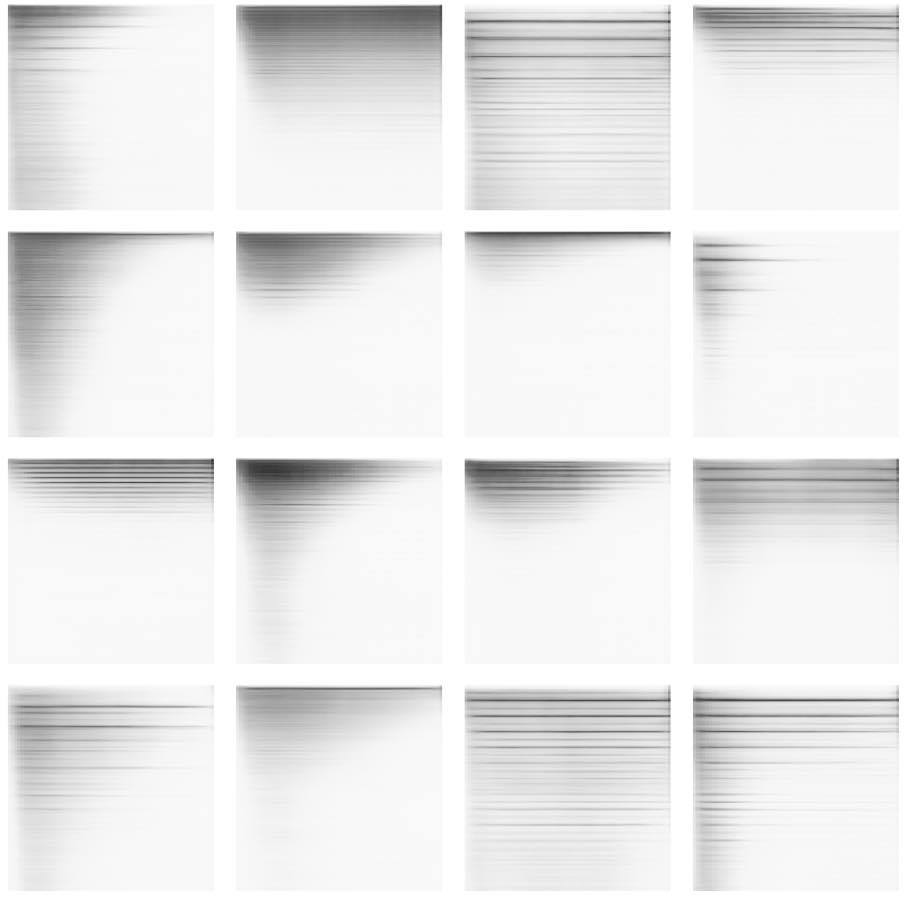
\includegraphics[width=0.9\textwidth]{gan.jpg}
	\caption{Spectrogram images generated by mode regularized generative adversarial network (MRGAN) %\cite{che2016mrgan} trained on instrumental sounds of Vienna symphonic library
	}\label{fig:gan}
\end{figure}

Future work in this project includes quantifying how the manifold learned by the GAN is informative in predicting various qualities of the sound, by combining the model with other GAN variants like InfoGAN \cite{chen2016infogan} or ACGAN \cite{odena2016acgan}.
Using NSynth dataset will also help in getting more insights of GAN's ability, since it is more organized and comes with more consistent annotations than Vienna Symphonic Library.


%!TEX root = ../dissertation.tex

\graphicspath{{7-conclusions/figures/}}

\chapter{Conclusions}
\label{ch:conclusions}

By combining deep learning's prodigious capacity to process multimedia data and the practically unlimited source of training data generated by software instruments and data augmentation, this proposal has presented a concrete plan toward a better automatic music transcription system.
Many data-driven methods for music information retrieval have shown that they can perform better than the traditional, heuristic-based methods when provided with enough data for training, and this work will develop further on that, with the help of deep generative models and the huge scale of training data.
These have been only very recently made possible, because of the availability of hardware and software for deep learning at the required scale, as well as the success of the deep generative models especially generative adversarial networks.
This leads to the conclusion that all of the hardware, software, techniques, and the data are pointing to the possibility of deep generative models for automatic music transcription, opening an era for automatic music transcription research.



%: ----------------------- bibliography ------------------------
{
\onehalfspacing
%\renewcommand{\bibfont}{\small}
%\renewcommand{\bibname}{Bibliography} % changes the header; default: Bibliography
%\printbibliography
\small
\bibliography{library/library} 
}

%: ----------------------- appendices --------------------------
% \appendixbegin
% \appendix

\chapter{Brownie tootsie roll lollipop cookie}
\label{adx:a}

\doublespacing

Oat cake pudding sweet lemon drops gummies cookie. 
Dragee lollipop ice cream apple pie sweet roll brownie. 
Lollipop marshmallow jelly beans marzipan sugar plum chupa chups caramels toffee. 
Croissant icing chocolate cake oat cake muffin powder tart. 
Croissant wafer dessert pudding cupcake croissant. 
Cheesecake wafer sugar plum danish. 
Liquorice powder sesame snaps.


%: --------------------------- index ---------------------------
% \clearpage
% \begin{footnotesize}
% \cleardoublepage % ensure the right page
% \phantomsection % sets an anchor
% \printindex
% \end{footnotesize}

\end{document}
